%%%%%%%%%%%%%%%%%%%%%%%%%%%%%%%%%%%%%%%%%%%%%%%

% Start with going to Settings/packages.tex and change the pdftitle and pdfauthor variables.

% Then make changes to pages in the Content folder, such as abstract, acknowledgement, declaration, supervisor and titlepage.

% Add your citations in the BibTex format in the citation.bib file. These can be found via the publisher website.

% Finally, add your content to chapters and appendices. Read all of them first as there might be some command explained there that you don't know. Additionally, add your figures to the Figure folder to keep them organised.

% Keep adding new chapters and appendices at their relevant places.

%%%%%%%%%%%%%%%%%%%%%%%%%%%%%%%%%%%%%%%%%%%%%%%

%% document class
\documentclass[12pt, a4paper, twoside]{report}

\usepackage{subfiles}
\usepackage{hyperref}
\usepackage{adjustbox}
\usepackage{float}
\usepackage{chngcntr}
\counterwithout{figure}{chapter}
\counterwithout{table}{chapter}
\usepackage{verbatim}



%% packages
%------------------------------------------------------------------------------------
%	PACKAGES AND OTHER DOCUMENT CONFIGURATIONS
%-------------------------------------------------------------------------------------

\usepackage{xcolor} % Required for specifying custom colours
\definecolor{grey}{rgb}{0.9,0.9,0.9} % Colour of the box surrounding the title

\usepackage[utf8]{inputenc} % Required for inputting international characters
\usepackage[T1]{fontenc} % Output font encoding for international characters
\usepackage{graphicx} % used for \includegraphics

\usepackage{blindtext} % used for dummy texts
\usepackage{amsmath} % used for \eqref to refer to any labeled math equation
\usepackage{amssymb} % used for mathematical symbols
\usepackage{lettrine}

%% \usepackage{makeidx}
%% \makeindex

%\usepackage[ backend=biber, citestyle=authoryear-comp, sorting=ynt]{biblatex}
\usepackage[sort]{natbib}
\bibliographystyle{abbrvnat}
\setcitestyle{authoryear,open={(},close={)}} %Citation-related commands

\usepackage{epigraph}

\usepackage{titlesec, blindtext, color}
\definecolor{gray75}{gray}{0.75}
\newcommand{\hsp}{\hspace{20pt}}
\titleformat{\chapter}[hang]{\Huge\bfseries}{\thechapter\hsp\textcolor{gray75}{|}\hsp}{0pt}{\Huge\bfseries}[\headrule]

\usepackage[colorlinks=True, breaklinks]{hyperref} % to add links
%% \usepackage[hyphenbreaks]{breakurl} % break long urls
\renewcommand{\figureautorefname}{Fig}
\renewcommand{\equationautorefname}{Eq}

\definecolor{c1}{rgb}{0,0.3,0.9}
\hypersetup{
    linkcolor={c1},
    citecolor={c1},
    urlcolor={c1},
    pdftitle  = {BTP - 180106007},
    pdfauthor = {Aditi Madkaikar}
}
\usepackage{lineno}
\usepackage{url}

\usepackage{caption}
\usepackage[toc,page]{appendix}
\usepackage{subfig}
\usepackage{multirow}
\usepackage{array}
\usepackage{multirow}
\usepackage{booktabs}
\usepackage{graphicx}
\usepackage{changepage}
\usepackage{subfigure}

\usepackage{float} % For H placement specifier
\usepackage{wrapfig}

\usepackage{graphicx}
\usepackage{subcaption}
\usepackage{float}
\usepackage{longtable}
%%\renewcommand{\baselinestretch}{}




\renewcommand{\labelenumi}{\arabic{enumi}.}
\usepackage{setspace}
\usepackage{hyperref}
\hypersetup{
    colorlinks=true,    % 将链接设置为颜色而不是方框
    linkcolor=black,    % 链接的颜色
    citecolor=black,    % 引用链接的颜色
    urlcolor=black      % URL链接的颜色
}
\usepackage{hyperref}




\newcommand{\HRule}{\rule{\linewidth}{0.5mm}} % Defines a new command for the horizontal lines, change thickness here

\newcommand{\quickwordcount}[1]{%
    \immediate\write18{texcount -1 -sum -merge #1.tex > #1-words}%
    \input{#1-words}words%
}

\usepackage{parskip}

\usepackage{datetime}
\newdateformat{monthyeardate}{\monthname[\THEMONTH] \THEYEAR}


%\addbibresource{Content/citation.bib}

%% page settings
%-------------------------------------------------------------------------------------
%	PAGE SETTINGS
%-------------------------------------------------------------------------------------

\usepackage[right=2cm, left=2cm, top=2.5cm, bottom=2cm]{geometry}
\parindent=0cm
\sloppy

\hyphenation{}
\hyphenpenalty=10000
\exhyphenpenalty=10000

\usepackage{fancyhdr}
\setlength{\headheight}{15pt}

\usepackage{setspace}

% \setcounter{secnumdepth}{0}
\renewcommand{\theenumi}{\alph{enumi}}


% Title of the project
\title{Revealing temporal trends in UK STEM funding}

\begin{document}


%%%%%%%%%%%%%%%%%%%%%%%%%%%%%%%%%%%%%%%%%%%%%%%
%%%%%%%%%%%%%%%%%%%%%%%%%%%%%%%%%%%%%%%%%%%%%%%

%----------------------------------------------------------------------------------
%	TITLE PAGE
%----------------------------------------------------------------------------------

\begin{titlepage} % Suppresses displaying the page number on the title page and the subsequent page counts as page 1
%--------------------------------------------------------------------------
    %	LOGO SECTION
    %--------------------------------------------------------------------------
    
    
\includegraphics[width=7cm]{Figures/collegeLogo.png} % Include a department/university logo
     
    %--------------------------------------------------------------------------
    
    \center % Center everything on the page
    
    %--------------------------------------------------------------------------
    %	HEADING SECTIONS
    %--------------------------------------------------------------------------
    \vspace{1cm}
    \quad\\[1cm]
    \textsc{\Large Imperial College London}\\[0.5cm] % Name of your university/college
    \textsc{\Large Department of Life Sciences}\\[0.5cm]
  
     
    %--------------------------------------------------------------------------
    %	TITLE SECTION
    %--------------------------------------------------------------------------
    \vspace{1cm}
    \makeatletter
    \HRule \\[0.4cm]
    { \huge \bfseries \@title}\\[0.4cm] % Title of your document
    \HRule \\[1cm]
     
    %--------------------------------------------------------------------------
    %	AUTHOR SECTION
    %--------------------------------------------------------------------------
    \vspace{1cm}
    \begin{minipage}{0.5\textwidth}
    \begin{flushleft} \large
    \emph{Author:} Hanyi Jiang \\
    \emph{CID:} 02281166\\
    \emph{email:} hj22@ic.ac.uk
    \end{flushleft}
    \end{minipage}
    ~
    \begin{minipage}{0.4\textwidth}
    \begin{flushright} \large
    % Supervisor's Name
    \emph{Supervisor:} \\
    Samraat Pawar
    s.pawar@imperial.ac.uk\\[1.2em]
    \end{flushright}
    \end{minipage}\\[2.5cm]
    \makeatother
    
    \vspace{3cm}
    %--------------------------------------------------------------------------
    %	DATE SECTION
    %--------------------------------------------------------------------------
    \quickwordcount{main}\\
    
    
    {\large A thesis submitted in partial fulfillment for the degree of}\\[0.1cm]
    \large Master of Research at Imperial College London\\[0.1cm]
    \textsc{\large \emph{Submitted for MSc Computational Methods in Ecology and Evolution}}\\[0.2cm] % Minor heading such as course title
    {\large \monthyeardate\today}\\ % Date
   % {\large \ CMEE coursework }\\[0.5cm] %emph{CMEEs} for italics
    
    
    \vfill % Fill the rest of the page with whitespace
	
\end{titlepage}
%\thispagestyle{empty}
%%\cleardoublepage

\pagenumbering{roman}

%\input{Content/supervisor.tex}

%%\cleardoublepage

%%\begin{center}
    \fontsize{20pt}{25pt}\selectfont
    \textbf{Declaration}
\end{center}
\vspace{1.5cm}




The data of the whole project was given by Flávia Bellotto Trigo (f.bellotto-trigo18@imperial.ac.uk). The author of the report, Hanyi Jiang, is responsible for data processing. The initial version of the code for this project was derived from Flavia. The author of this report, Hanyi, made significant modifications and additions to the code to fulfill the analysis requirements. 




%%\cleardoublepage

\begin{center}
    \fontsize{20pt}{25pt}\selectfont
    \textbf{Declaration}
\end{center}
\vspace{1.5cm}




The data of the whole project was given by Flávia Bellotto Trigo (f.bellotto-trigo18@imperial.ac.uk). The author of the report, Hanyi Jiang, is responsible for data processing. The initial version of the code for this project was derived from Flavia. The author of this report, Hanyi, made significant modifications and additions to the code to fulfill the analysis requirements. 



\newpage
\begin{center}
    \fontsize{20pt}{25pt}\selectfont
    \textbf{Acknowledgement}
\end{center}

\vspace{1.5cm}

I would like to express my sincere gratitude to my supervisor, Samraat Pawar and Flávia Bellotto Trigo, Imperial College London for invaluable guidance, expertise and support throughout the duration of the project.


\vspace{2cm}

% \parbox[t]{\textwidth}{
%     % Horizontal line, first argument width, second thickness
%     % Box to inset this section slightly
% 	\raggedleft % Right align the text
% 	Sincerely, \\
% 	Your name
% }

%%\cleardoublepage
\begin{spacing}{0.85}
    \tableofcontents
\end{spacing}
%%\cleardoublepage
\newpage

\phantomsection
\addcontentsline{toc}{chapter}{List of Figures}
\listoffigures

% % \newpage
\begingroup
\let\clearpage\relax
\phantomsection
\addcontentsline{toc}{chapter}{List of Tables}
\listoftables
\endgroup


\newpage
\phantomsection
\addcontentsline{toc}{chapter}{Abstract}

% Try to keep the abstract page on an odd numbered page. If your table of contents spill over to two pages, just remove the \cleardoublepage after \tableofcontents and add it here. That is how you can keep the abstract page on an odd numbered page.
% This is to help you organise the report when you print it out. Everything will start on the right side, which is aesthetic.
\begin{abstract}


\linenumbers 
Countries worldwide have always paid continuous attention to and supported scientific research. Based on our daily experience, it seems that fields such as biology or AI have received a lot of attention recently, but this lacks research support. So what does the current scientific landscape look like? And how did it arrive at the current pattern?

I take the UK Research and Innovation (UKRI) as a case study to analyze investment directions and structures, aiming to yield profound insights into the funding landscape and its development process. Employing a data-driven approach, I leverage machine learning techniques, particularly the Mallet Latent Dirichlet Allocation (LDA).\\

The ultimate discovery underscores a pronounced tendency to allocate funds towards applied and natural sciences, reflecting their paramount significance within the research agenda. During the 20 years of analysis, in each three-year period, more than 80\% of the invested projects belong to applied and natural science. 2022-2024, according to incomplete statistics, the two companies received 6,785,877,536 pounds of funding, accounting for 92.15\% of the total expenditure funding amount. Furthermore, ecology has consistently received significant attention and continuous funding over the years. During the period from 2016 to 2018, it secured a total funding of £108,990,748. This amount positioned ecology as the second highest-funded field within natural sciences. Nevertheless, the intricacies of these domains have given rise to many specialized orientations. Alternatively, while receiving fewer and comparatively modest allocations in the social sciences domain, public policy occupies a dominant position. Apart from the period between 2010 and 2012, during which business projects also received funding, funds were exclusively allocated to Public Policy within the realm of social sciences in all other years.\\

By analyzing the dynamic funding allocation in UKRI, I unveil the ever-evolving priorities and prospects within the funding landscape, revealing the history of scientific development and possible future development trends.\\







\end{abstract}


%%\cleardoublepage

%%%%%%%%%%%%%%%%%%%%%%%%%%%%%%%%%%%%%%%%%%%%%%%
%%%%%%%%%%%%%%%%%%%%%%%%%%%%%%%%%%%%%%%%%%%%%%%
\newpage
\pagestyle{fancy}
\fancyhf{}
%\lhead[\leftmark]{}
\chead[]{}
%\rhead[]{\rightmark}
\fancyfoot[LE, RO]{\thepage}
\setcounter{footnote}{-1}

\pagenumbering{arabic}

\chapter{Introduction}
\linenumbers 
\lettrine[lines=1]{I}{n}
recent years, humankind has faced many daunting challenges, including  military conflicts, rising sea levels gradually making some cities disappear, pandemics, noncommunicable diseases, dwindling resources, and so forth, and are also working hard to iterate technology. Countries have reached a record high of almost US \$1.7 trillion in spending on technological innovation and scientific research \citep{RN16}. \\


Recently, research remains at the forefront of understanding and addressing these complex problems. The foundation of any successful research project relies on innovative ideas and meticulous execution \citep{neema2021research}. Conducting research, especially in fields like wet laboratory science or large-scale epidemiological studies, demands substantial funding to cover tangible and intangible costs \citep{schembri2018wasp}. Therefore, even though the process of applying for funding is by no means an easy task and is considerably daunting and time-consuming, with EU research programs, for example, EU research (such as Horizon 2020), application success rates are only around 15\% \citep{schembri2018wasp}, researchers generally opt to seek research funding to ensure the smooth operation of their research projects. Encouragingly, governments, universities, and nonprofit organizations recognize the pivotal role of research and development (R\&D) in driving economic growth, job creation, national security, environmental protection, and knowledge expansion \citep{sargent2017global}. \\

In 2020, global R\&D expenditures reached \$2.352 trillion \citep{sargent2017global}. The 10 largest R\&D-funding countries of 2020 accounted for \$1.999 trillion in R\&D expenditures \citep{sargent2017global}. Such substantial investments highlight the commitment to foster research and innovation. In fact, securing adequate funding is crucial to fueling the relentless pursuit of scientific breakthroughs. For instance, Gush et al.'s findings indicate that funding is correlated with a 6-15\% increase in publications and a 22-26\% increase in citation-weighted papers for research teams \citep{gush2018effect}.\\


In 2021, The UK government’s net expenditure on research and development (R\&D), excluding EU contributions, remained at \pounds14.0 billion. Within the UK, research funding takes two primary forms: commercial and non-commercial, with the latter dominating the landscape. Non-commercial funding sources encompass research charities, national academies, various government departments, and the United Kingdom Research and Innovation (UKRI).\\

Among these organizations, UKRI is UK's most significant public funder of research and innovation, principally funded through the Science Budget by the Department for Business, Energy and Industrial Strategy (BEIS). According to UKRI Annual Report and Accounts 2021-22, they invest more than £8 billion annually to advance our understanding of people and the world around us and deliver benefits for society, the economy, and the environment. \\

From everyday conversations and the information we gather from online news, we might form a rough perception that the field of science and technology tends to secure a higher frequency of funding for projects. However, these notions are not substantiated and are essentially intuitive assumptions. Moreover, as time progresses, the emergence of novel discoveries continuously challenges or validates our existing beliefs, potentially reshaping the landscape of future funding allocation. This inevitably prompts the question: Can discoveries wield a fresh influence on funding arrangements?\\

Hence, through a comprehensive analysis of investment patterns, I can uncover the focal points of institutions and gain insights into the developmental trajectories of various specialized domains. Furthermore, this analysis provides a more precise understanding of the rise and fall of various domains and their specific manifestations in terms of funding allocation. Understanding research funding trends carries immense significance for researchers, policymakers, and funding agencies. By unraveling the ever-changing landscape of research investment, people can identify shifts in research priorities and potential areas of innovation. Such insights will empower us to address contemporary challenges effectively and adapt research strategies for future endeavors.\\

Notably, I seek to address the following key research questions:

\begin{enumerate}
  \item Evolution of Research Funding Priorities: How have research funding priorities evolved across different disciplines and industries? 
  \item Emerging Research Areas: What emerging research areas have gained prominence recently, and how do they align with societal needs and technological advancements?
  \item Drivers of Fluctuations: What are the driving factors behind fluctuations in research attention to specific themes in different periods?\\
  \item What is the funding trend for ecology and evolution?\\
 
\end{enumerate}

I will employ AI-driven methods to process and visualize the data, revealing patterns and connections between funding allocation and significant temporal factors. Monitoring and comprehending shifts in research investment will empower me to effectively tackle current challenges and tailor research strategies for upcoming pursuits.\\
\chapter{Methods}
\lettrine[lines=1]{M}{y}
primary objective based on an extensive dataset encompassing funded projects by UKRI throughout the UK, comprising crucial information such as project titles, abstracts, and corresponding funding amounts. Armed with these comprehensive data, I employed topic analysis methods to ascertain the distinct research domains to which they pertained. This analytical endeavor was intended to discover the evolving landscape of research focus across various disciplines, revealing prominent areas that have garnered substantial support from UKRI-funded programs over the past few decades. By scrutinizing the ever-evolving patterns and dominant themes, I aimed to gain valuable insights into the investment preferences and strategic directions pursued by research funding agencies, particularly UKRI. \\

\section*{Data Preprocessing and Preparation}
The available data for analysis consists of UKRI records spanning from 1973 to 2023. The minimum data requirement includes project titles, start dates, titles, abstracts, funding amounts, and all other available project-specific metadata. \\

During the data preprocessing stage, I made various attempts to guarantee the efficiency of information filtering and subject analysis in the subsequent phases. To begin with, I grouped all the available data from 1973 into five-year intervals. Each group consisted of two parts: the title summary, comprising project summaries and project IDs, and the metadata part, encompassing all other project-related details.\\

However, upon completing the grouping, I encountered an issue with the datasets for 1973-1977, 1978-1983, 1984-1988, and 1989-1993. These groups had very limited data, with the number of projects being less than 100, which rendered them less valuable for meaningful research. Similarly, the number of projects in 1999-2003 did not exceed 1,000. Considering that the actual number of funded projects may be substantially higher than those reflected in the data, I discard data before 2004 and focus solely on projects from 2004 to 2023.\\

Under such circumstances, to enhance analysis accuracy, I further reduced the time interval and regrouped the data every three years. This adjustment would yield more informative and comprehensive datasets for in-depth subject analysis and allow for a more robust examination of trends and research preferences in recent years.\\

After grouping the data, I started to process the data file formally. I have implemented the following to remove noise in the dataset.

\begin{enumerate}
  \item Tokenization: Breaking down raw text into individual words
  \item Removing punctuation and stop words*
  \item Lemmatization: remove inflectional endings only and return the base or dictionary form of a word \citep{kurt2020topic}.
  \item Remove incomplete projects from the dataset to ensure data quality and reliability.
  \item Removes words that appear less than 20 times
  \item Removes words that appear in 80\% of the documents
\end{enumerate}

*Stop words are common words frequently used in natural language but usually lack practical meaning or have no significant impact on text analysis tasks. Since these words do not usually carry specific semantic information, they are often ignored or removed from the text in tasks to reduce data dimensions, improve processing efficiency, and help focus on meaningful keywords or phrases \citep{rajaraman2011mining}.

\section*{Preparing Topic Numbers for Mallet LDA}

The current challenge lies in the abundance of unstructured abstracts  in the dataset, making extracting relevant and necessary information difficult. To address this, I opted for topic modeling techniques from the field of text mining. \\

Topic modeling is a valuable tool in statistics and natural language processing, employing a statistical model to unveil abstract "topics" in a collection of documents. This powerful text-mining approach enables the discovery of hidden semantic structures within the text, offering valuable insights into the underlying themes and concepts in the analyzed documents \citep{arun2010finding}. To be more specific, a topic model is a probabilistic model used to discover topics, or latent structures, across a collection of documents \citep{saxton2018gentle}. There are many approaches for obtaining topics from a text, such as – Term Frequency and Inverse Document Frequency. Topic modeling encompasses various techniques, including four of the most popular approaches: LDA, Mallet LDA, STM, and HDP \citep{egger2022topic}.\\

Latent Dirichlet Allocation (LDA), an unsupervised machine learning approach, was proposed by Blei, David M., Ng, Andrew Y., and Jordan in 2003, which is a powerful algorithm that enables exploring and discovering latent topics within extensive collections of text known as corpora \citep{chipidza2022topic}. LDA can infer the topic of each document in the form of probability distribution, so that after analyzing some documents to extract their topic distribution, topic clustering or text classification can be performed according to the topic distribution \citep{blei2012probabilistic}.In LDA (Latent Dirichlet Allocation), the Bag-of-Words model is employed, commonly known as the "bag-of-words" model. In this model, each document is represented as a collection of words, disregarding their order of appearance. \\

Mallet LDA and LDA are highly correlated. The MALLET topic modeling toolkit contains efficient, sampling-based implementations of Latent Dirichlet Allocation, Pachinko Allocation, and Hierarchical LDA \citep{mallet}. According to the experiences of Senol Kurt and the authors of the Gensim tutorial, utilizing the MALLET package (with Python wrapper) to implement the LDA approach for topic generation has been found to produce superior results \citep{kurt2020topic}. Hence, I have adopted the Mallet LDA approach for my project.\\

To determine the number of topics for the Mallet LDA model, I employed the \texttt{mallet evaluate-topics} command to analyze the model's performance across a range of topic numbers, from 50 to 400, with intervals of 50. I used perplexity as the evaluation criterion. Perplexity measures the model's ability to predict unseen test data, normalized by the number of words in the evaluation. The perplexity formula is defined as follows:
\begin{equation}
PP(W) = \left( P(W_1W_2, \ldots, W_m)^{-\frac{1}{m}} \right)
\end{equation}

where $PP$ represents perplexity, $W$ refers to the words in the document, and $P$ denotes the probability estimate assigned to the document words. An LDA model with a specific number of topics that yields the minimum perplexity value is considered the optimal model \citep{neishabouri2020reliability}. \\

Afterward, I utilized the "mallet run cc.mallet.util.DocumentLengths" command to calculate the lengths of documents in the test set and saved the results to a file. Following this, I implemented a loop to iterate through different numbers of topics, ranging from 50 to 400 with increments of 25. For each topic number, I utilized the "mallet train-topics" command to train the topic model, generating three files: the diagnostic file, the inferencer file, and the topics-state.gz file. The inferencer file contains the necessary parameters for inferring topics in new documents, while the topics-state.gz file includes the training data along with all the inferred parameters, which leads to the fact that the inferencer file is much smaller than the topics-state.gz file.\\

On the other hand, the diagnostic files contain essential information under each topic number, such as the topic ID and relevant statistical metrics, including word count, probability, cumulative probability, document count, word length, coherence, and more. Among them, the coherence metric measures the semantic similarity between high-scoring words in a topic, providing insights into the quality and coherence of the generated topics \citep{kapadia2022evaluate}.\\

Perplexity is one of the most widely used evaluation metrics for language models. Hence, I leveraged the "mallet evaluate-topics" command to assess the performance of the model on the test set and derive its perplexity value. In essence, perplexity focuses on the log-likelihood aspect, providing an indication of how probable new unseen data is when considering the model that was previously learned. In other words, it measures how effectively the model captures the statistics of the held-out data \citep{kapadia2022evaluate}. A lower perplexity value indicates a higher level of coherence and a better-performing model in representing the underlying patterns of the unseen data \citep{neishabouri2020reliability}.\\

After the evaluation, I found that the model with 50 topics achieved the lowest perplexity value of -2.277E7. Therefore, I determined that setting the number of topics to 50 for the subsequent topic inferring process would be the most suitable choice.\\

\section*{Topic Modeling Using Mallet LDA}
Once the number of topics is determined, which is 50, the process of topic inference begins with the "mallet infer-topics" command. This command utilizes the previously trained inferencer file as input and generates the topic distribution table. In this table, each row corresponds to a project abstract, and each column represents a topic, with the values indicating the degree of association between each abstract and the different topics. This table effectively illustrates the association level between each abstract and the various topics, facilitating subsequent topic analysis and text comprehension.\\

Next, I used xml.etree.ElementTree to parse the diagnostic information from the XML file generated by Mallet, which contained details about the 50-topic model, allowing me to obtain the specific vocabulary associated with each topic.\\

In the penultimate step, I leveraged the power of ChatGPT to gain deeper insights and understanding from the topic-related words obtained in the previous steps. By reading and parsing the XML file containing the diagnostic information of the Mallet-generated topic model with 50 topics, I extracted the specific vocabulary associated with each topic.\\

With integrating these topic-related words into ChatGPT, I harnessed its capabilities to derive precise directions and valuable insights based on the given topic words. This fusion of Mallet LDA and ChatGPT enabled me to effectively explore and comprehend the underlying themes and concepts concealed within the extensive collection of abstracts.\\

\section*{Topic Analysis and Funding Trends Evaluation}
As a final step, I comprehensively evaluated the topic distribution table. Each row in the file represents a distinct project, with the subsequent 50 columns containing probabilities associated with different topics. By employing Python's Pandas package, I meticulously analyzed the data on the dominant topic for each project based on the highest probability. Additionally, I derived insights into the distribution of projects across various topics and compiled an overview of the cumulative funding received by projects associated with each topic. This approach provided valuable insights into the thematic landscape and funding trends within the dataset.



\chapter{Results}
\lettrine[lines=1]{O}{ver}
 a span of 51 years, from 1973 to 2024, prominent themes have emerged and endured. Notably, biology, chemistry, environmental science, and materials science have consistently dominated the landscape, showcasing their enduring significance. 
%TC:ignore
\begin{table}[H]

    \caption{Science Takes Center Stage (1973-2024)}
    \label{tab: Topic List}

    \begin{adjustbox}{width=\textwidth} 
        \begin{tabular}{ *{5}{c} } 

            \midrule
            Material Science	&	Physics	&	Business	&	Developmental Biology	&	Political Science	\\
Medicine	&	Imaging Techniques	&	Automotive	&	Climate Science	&	Sensor Technology	\\
Epidemiology	&	Media Studies	&	Environmental Science	&	Development	&	Chemistry	\\
Philosophy	&	Infrastructure	&	Neuroscience	&	Ecology	&	Climate Science	\\
Microbiology	&	Particle Physics	&	Evolutionary Biology	&	Optics	&	Quantum Physics	\\
Biochemistry	&	Statistics	&	Computer Science	&	Manufacturing	&	Agriculture	\\
Healthcare	&	Machine Learning	&	Public Health	&	Networking	&	Astronomy	\\
Material Science	&	Biochemistry	&	Pediatrics	&	Immunology	&	Food Science	\\
Education	&	Oncology	&	Waste Management	&	Electronics	&	Oceanography	\\
Molecular Biology	&	Modeling	&	Mathematics	&	Geology	&	Surgery	\\

            \bottomrule
        \end{tabular}
    \end{adjustbox}
\end{table}
%TC:endignore
While this analysis provides valuable insights, it's important to acknowledge that the vast temporal scope might limit the depth of information attained. \\

I partitioned the metadata into consecutive three-year periods to gain deeper insights into the evolving landscape for a more concentrated exploration of the dominant trends and subjects influencing research and innovation within these specific timeframes. This focused examination of shorter intervals will provide a finer-grained and more intricate viewpoint. 

I have made six significant findings by analyzing and consolidating each triennial topic. 

\begin{enumerate}

  \item Sustained Importance: The topics of Environmental Science, Computer Science, Data Science, Ecology, Biology, and Training are consistently present throughout various periods, emphasizing their enduring significance and impact.

  \item Transient Topics: Some projects have emerged briefly during specific years, such as video games and supply chain disruptions in 2019-2021.

  \item Environment and Sustainable Development: During 2016-2018, there was a pinnacle of concern regarding environmental issues. The prevailing topics of that era were predominantly associated with the environment, including environmental science, earth science, ecology, energy materials, waste management, energy transfer, earth and geology, etc.

  \item Data science, computer science, and machine learning have repeatedly emerged at various time intervals.

  \item Limited Presence of Social Sciences: Public policy is a prominent funded focus within social science.

  \item Certain topics experienced fluctuations in attention across different years. For instance, Particle Physics was prominent in earlier years but waned later.\\
  
\end{enumerate}
%TC:ignore
\begin{table}[H]

    \caption{Topic List}
    \label{tab: Topic List}

    \begin{adjustbox}{width=\textwidth} 
        \begin{tabular}{ *{5}{c} } 
            \toprule
            2010-2012 & 2013-2015 & 2016-2018 & 2019-2021 & 2022-2024 \\
            \midrule
            Imaging	&	Machine Learning	&	Human-Computer Interaction	&	Problem Solving	&	Environmental Engineering	\\
Diagnostic Technology	&	Medical Technology	&	Healthcare	&	Agriculture	&	Medical Science	\\
Computer Science	&	Automotive Engineering	&	Transportation	&	Genetics	&	Engineering	\\
Neuroscience	&	Environmental Science	&	Environmental Science	&	Particle Physics	&	Microbiology	\\
Electronics	&	Neuroscience	&	Neuroscience	&	Natural Hazards	&	Mathematics	\\
Materials Science	&	Climate Science	&	Earth Science	&	Climate Resilience	&	Sports Science	\\
Environmental Science	&	Environmental Monitoring	&	Sensors and Monitoring	&	Data sensing	&	Physics	\\
Atmospheric Science	&	Ecology	&	Ecology	&	Quantum Technology	&	Agriculture	\\
Oceanography	&	Cell Biology	&	Cell Biology	&	Astrophysics	&	Plant Science	\\
Analytical Chemistry	&	Fluid Dynamics	&	Particle Chemistry	&	Protein Structure	&	Molecular Biology	\\
Bioinformatics	&	Cybersecurity	&	Network Security	&	Medical Diagnostics	&	Health Science	\\
Pharmaceutical Science	&	Plant Science	&	Agriculture	&	Soil Ecology	&	Education	\\
Quantum Physics	&	Biochemistry	&	Molecular Biology	&	Infectious Disease	&	Environmental Science	\\
Climate Science	&	Fluid Mechanics	&	Fluid Dynamics	&	Wind Energy	&	Geology	\\
Human-Computer Interaction	&	Data Analysis	&	Ecology	&	Industry Training	&	Theoretical Physics	\\
Climate Science	&	Energy Systems	&	Quantum Science	&	Pandemic	&	Climate Science	\\
Automotive Engineering	&	Chemical Reactions	&	Materials Science	&	Modeling	&	Ecology	\\
Natural Disaster	&	Genetics	&	Chemical Reactions	&	Drug Development	&	Molecular Biology	\\
Evolutionary Biology	&	Materials Science	&	Genomics	&	Agriculture	&	Earth Science	\\
Particle Physics	&	Environmental Pollution	&	Energy Materials	&	Sustainable Transport Solutions	&	Astrophysics	\\
Technology Management	&	Medical Imaging	&	Environmental Pollution	&	Climate Change	&	Imaging	\\
Fluid Dynamics	&	Food Science	&	Imaging Techniques	&	Stem Cell Development	&	Data Analysis	\\
Education	&	Risk Assessment	&	Agriculture	&	Biodiversity	&	Physiology	\\
Geology	&	Microbiology	&	Disaster Management	&	Pollution Monitoring	&	Molecular Biology	\\
Astrophysics	&	Virology	&	Microbiology	&	Environmental Science	&	Computer Science	\\
Climate Science	&	Recycling	&	Infectious Diseases	&	Data Analysis	&	Microbiology	\\
Sensor Networks	&	Systems Modeling	&	Waste Management	&	Immune System	&	Material Science	\\
Theoretical Physics	&	Energy Management	&	Modeling	&	Machine Learning	&	Particle Physics	\\
Organic Chemistry	&	Plasma Physics	&	Energy Systems	&	Imaging	&	Medicine	\\
Materials Science	&	Astronomy	&	Plasma Physics	&	Geology	&	Astrophysics	\\
Ecology	&	Aircraft Engineering	&	Astronomy	&	Material Design	&	Engineering	\\
Infectious Disease	&	Aging	&	Aerospace Engineering	&	Public Policy	&	Geology	\\
Agriculture	&	Thermodynamics	&	Aging	&	Robotics	&	Health Science	\\
Public Policy	&	Material Engineering	&	Energy Transfer	&	Business	&	Particle Physics	\\
Cell Biology	&	Technology Innovation	&	Material Failure	&	Cybersecurity	&	Material Science	\\
Information Technology	&	Training	&	Technology	&	Particle Physics	&	Environmental Science	\\
Remote Sensing	&	Mathematics	&	Training	&	Drug Discovery	&	Computer Science	\\
Healthcare	&	Geology	&	Mathematics	&	Material Science	&	Cell Biology	\\
Ecology	&	Mathematics	&	Earth and Geology	&	Video Game	&	Chemistry	\\
Computational Science	&	Computer Science	&	Statistics	&	Fluid Dynamics	&	Mathematics	\\
Climate Modeling	&	Training	&	Computer Science	&	Mathematics	&	Climate Science	\\
Oncology	&	Molecular Biology	&	Vocational Training	&	Supply Chain	&	Neuroscience	\\
Molecular Biology	&	Cancer Research	&	Genetics	&	Chemical Synthesis	&	Public Policy	\\
Plant Breeding	&	Cardiovascular Diseases	&	Cancer Treatment	&	Clean Energy	&	Data Science	\\
Physiology	&	Semiconductor Technology	&	Medical Care	&	Public Health	&	Material Science	\\
Genetics	&	Data Analysis	&	Optics	&	Neurology	&	Control Systems	\\
Systems Biology	&	Particle Physics	&	Data Analysis	&	Aging	&	Energy Science	\\
Nutrition	&	Public Health	&	Particle Physics	&	Advanced Materials	&	Environmental Science	\\
Environmental Engineering	&	Cell Signaling	&	Public Health	&	Marine Environment	&	Hydrology	\\
Product Development	&	Physiology	&	Immunity	&	Ecosystem Biodiversity	&	Fluid Dynamics	\\
            \bottomrule
        \end{tabular}
    \end{adjustbox}

\end{table}
%TC:endignore
Some data entries in (table \ref{tab: Topic List}) are duplicated due to Mallet LDA's topic analysis, which treats vocabulary for each topic separately. However, similarities in topic direction can lead to duplicated content. I've integrated duplicated content in subsequent analyses to ensure accuracy and consistency.




\section*{Analysis Based on Project Number}
Building upon the systematic analysis and consolidation of each triennial topic, I conducted an in-depth examination of the prevailing thematic trends. I adopted a categorization framework inspired by Wikipedia's ``Outline of Academic Disciplines.'' This framework systematically classifies endeavors into five distinctive domains: Humanities, Social Science, Natural Science, Formal Science, and Applied Science. Applying this framework gave me a comprehensive perspective through which knowledge's intricate and multifaceted landscape could be thoroughly navigated and understood. 

Upon thorough analysis, it is clear that UKRI exhibits a pronounced concentration in its project selection, revealing a distinct inclination toward funding projects within Applied Science, closely trailed by Natural Science. Applied science is the use of the scientific method and knowledge obtained via conclusions from the method to attain practical goals \citep{bunge1966technology}, which usually have specific commercial objectives related to products, procedures, or services and deal with solving practical problems \citep{potter2015crime}. When it comes to natural science, it is entirely grounded in events and phenomena that occur naturally, encompassing two major categories: life sciences and physical sciences. Merriam-Webster's definition of natural science aligns with this, describing it as any scientific discipline concerned with matter, energy, and their interrelations and transformations or with objectively measurable phenomena \citep{ledoux2002defining}.\\

These two categories encompass a substantial array of subjects, including Material Science, Environmental Science, Microbiology, and Cell Biology – disciplines often characterized by their intensive need for experimentation and material resources, necessitating substantial funding. \\

Simultaneously, a select subset of Formal Science, such as Mathematics, Statistics, Computer Science, and certain Social Science projects, has garnered funding from UKRI. Regrettably, Humanities have garnered a notably diminished share of funding projects over these 21 years, rendering their presence comparatively inconspicuous when compared to the other four categories.\\


The correlation between UKRI's funding patterns and their 2022-2027 strategic priorities provides additional validation for these conclusions. The five strategic focal points, namely "Fostering Sustainable Environmental Practices," "Promoting Global Security and Resilience," "Enhancing Opportunities and Outcomes," "Ensuring Enhanced Health, Ageing, and Wellness," and "Combatting Infectious Threats," closely align with the domains of Applied Science and Natural Science, which have received significant funding. This congruence further underscores UKRI's deliberate strategy to address urgent global challenges and propel pragmatic solutions within these fields.
%TC:ignore
\begin{figure}[H]
    \centering
    \begin{minipage}{0.49\textwidth}
        \centering
        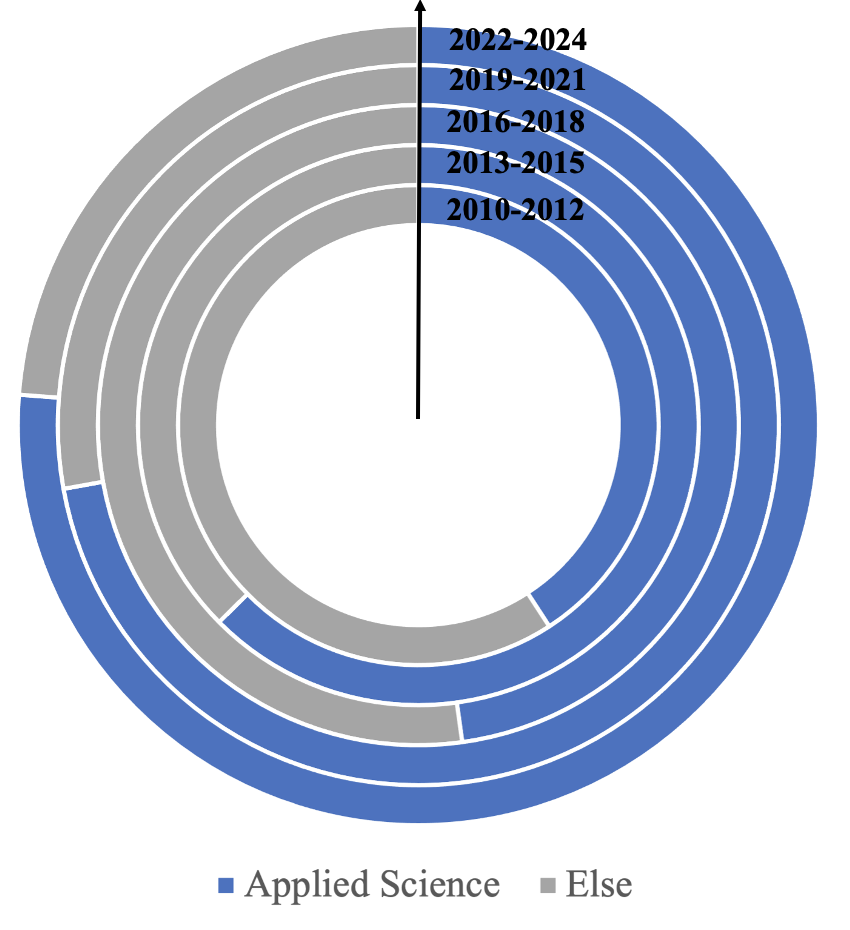
\includegraphics[width=\textwidth]{ProjectReportTemplate/Figures/Applied_Science.png}
      
    \end{minipage}
    \hfill
    \begin{minipage}{0.49\textwidth}
        \centering
        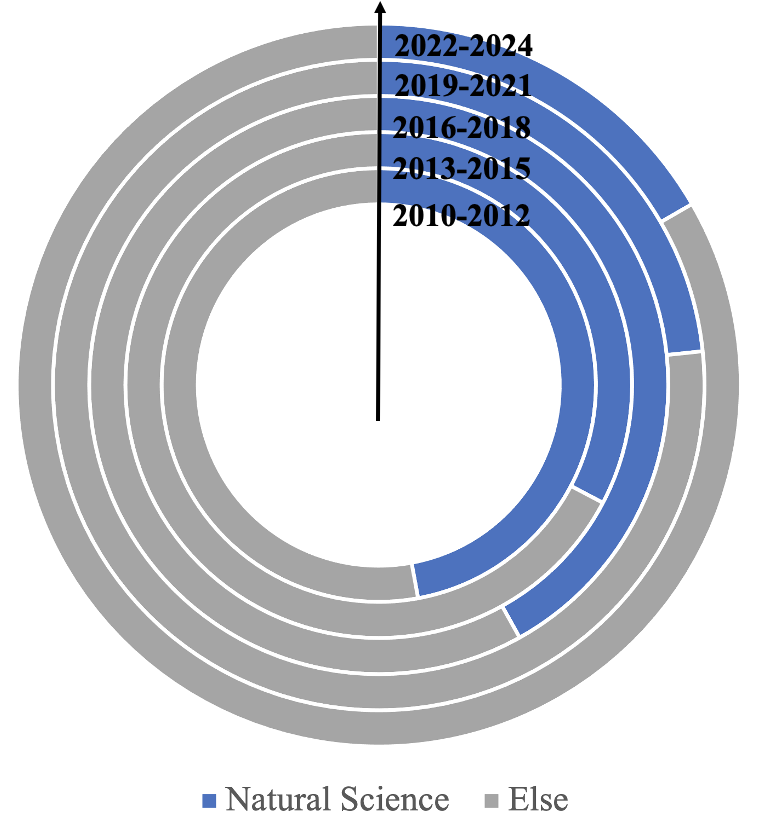
\includegraphics[width=\textwidth]{ProjectReportTemplate/Figures/Natural_Science.png}
       
    \end{minipage}
    
    \begin{minipage}{0.49\textwidth}
        \centering
        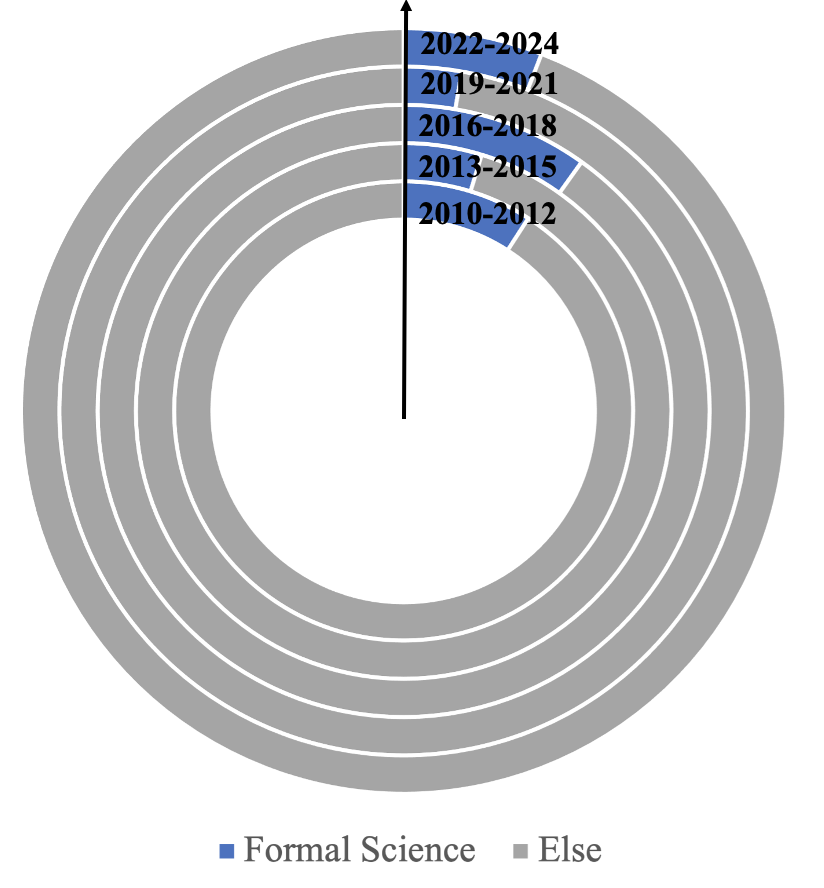
\includegraphics[width=\textwidth]{ProjectReportTemplate/Figures/Formal_Science.png}
    
    \end{minipage}
    \hfill
    \begin{minipage}{0.49\textwidth}
        \centering
        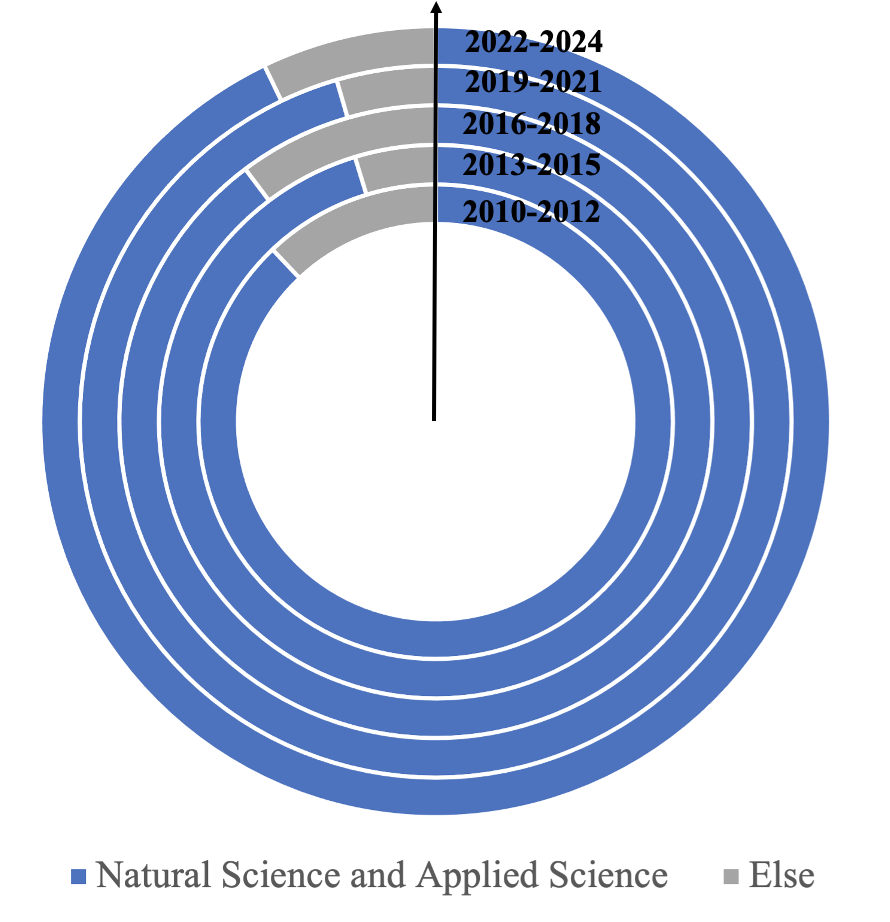
\includegraphics[width=\textwidth]{ProjectReportTemplate/Figures/Applied_Natural_Science.png}
     
    \end{minipage}
    \caption[Proportional Trends Shifting in Research Landscape]{The transition from the inner to the outer circle corresponds to the progression of time from past to present. While the evolution of applied science and natural science exhibits less distinct trends, it is noteworthy that these two domains consistently maintain their status as the most funded areas.}
    \label{fig:combined}
\end{figure}
%TC:endignore


Furthermore, within the realm of social sciences, funding has primarily directed its focus toward public policy. However, the quantity of projects received within the public policy field is comparatively remarkable. Across the periods of 2010-2012, 2019-2021, and 2022-2024, social science has witnessed support solely directed towards public policy. Also, in 2010-2012, 346 projects were funded under the public policy category, surpassing the funding count of any formal science topic and surpassing many themes within the natural science domain. Public policy has emerged as a cornerstone of social science, garnering substantial attention and resources.\\

Moreover, each triennial interval showcases standout topics that have surged ahead and captured substantial funding. For instance, in 2013-2015, "Automotive Engineering" within the Applied Science category witnessed a staggering 1117 funded projects, a testament to its robust prominence. Similarly, 2016-2018 witnessed a surge of funding in the "Material Science" domain, with an impressive tally of 1253 projects. Notably, 2019-2021 witnessed a crescendo in the "Applied Science - Public Health" category, with a significant surge of 1232 funded projects – a phenomenon that perhaps correlates with the emergence of the COVID-19 pandemic.\\

From 2022 to 2024, while Applied Science continues to receive the highest number of funded projects, its subdomains have noticeably decreased. The increase in the overall number of funded projects in Applied Science contrasts with the reduction in the diversity of its subdomains, suggesting a tendency toward consolidation within the Applied Science domain. To be specific, 68.75\% of the investment directions in applied science for 2022-2024 align with those invested during 2019-2021.\\

%TC:ignore
\begin{figure}[H]
    \centering
    \begin{minipage}{0.7\textwidth}
        \centering
        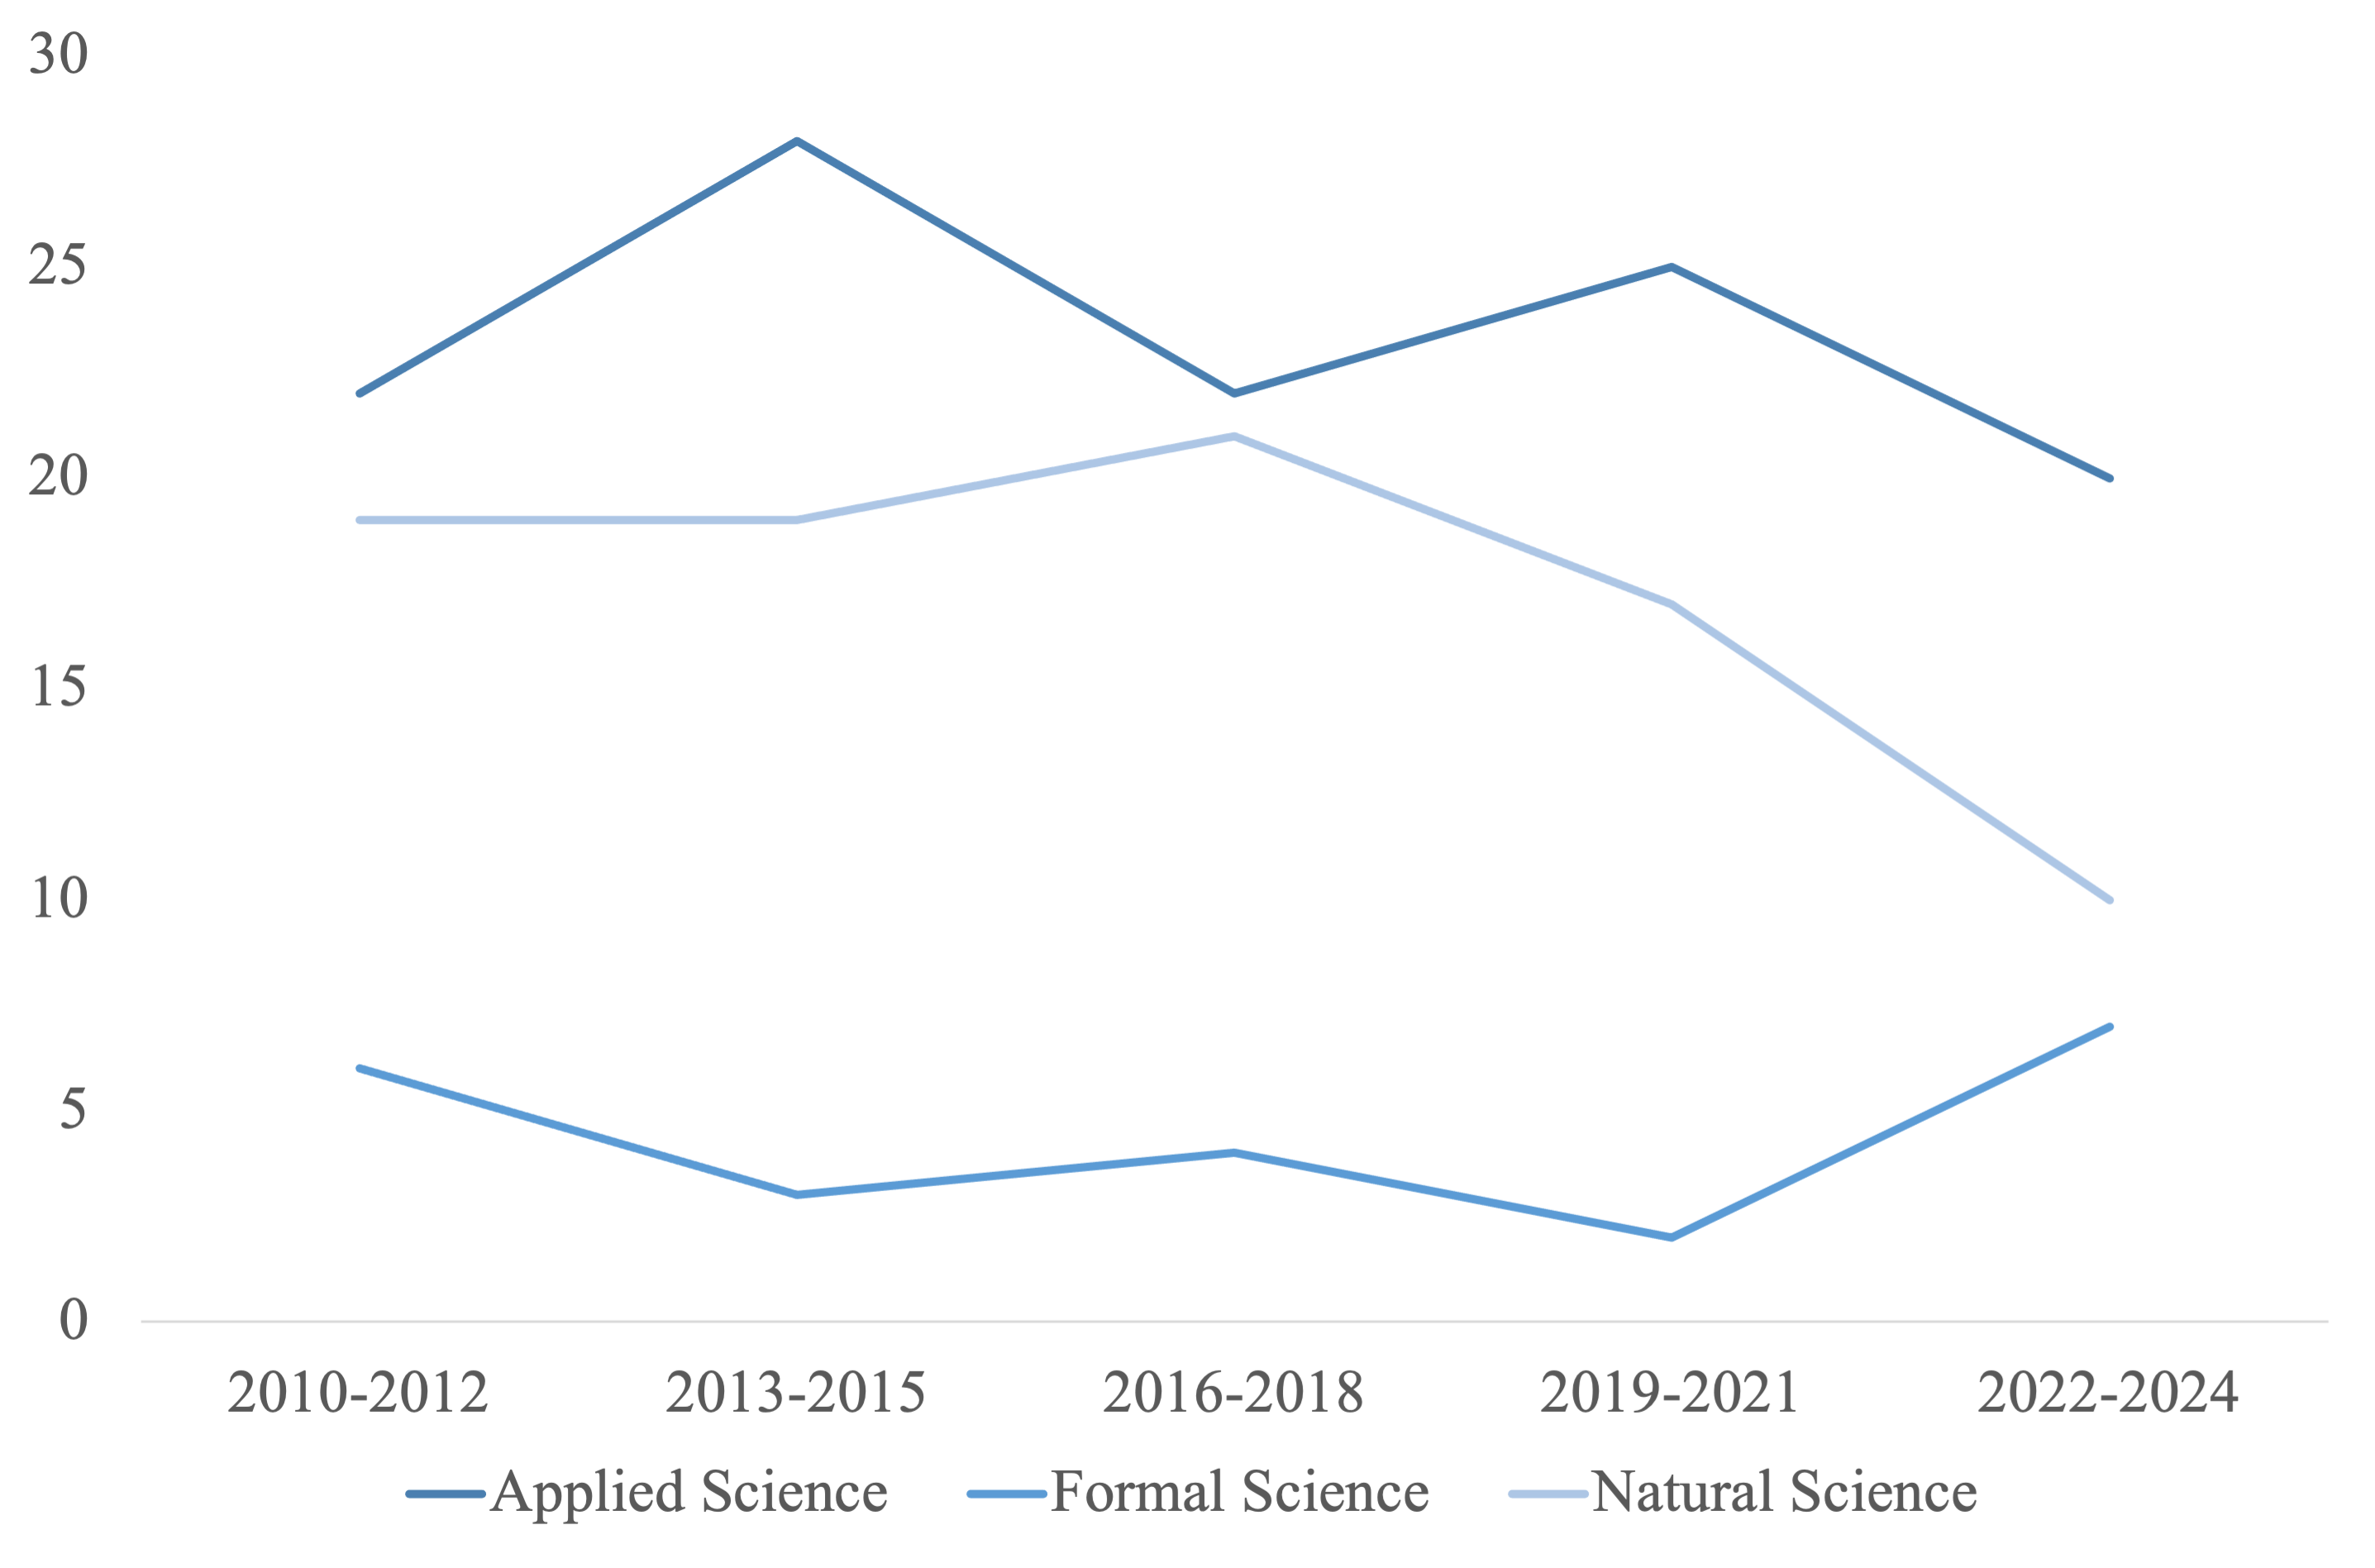
\includegraphics[width=\textwidth]{Figures/The number of subdomains within each category.png}
      
    \end{minipage}

    \begin{minipage}{0.7\textwidth}
        \centering
        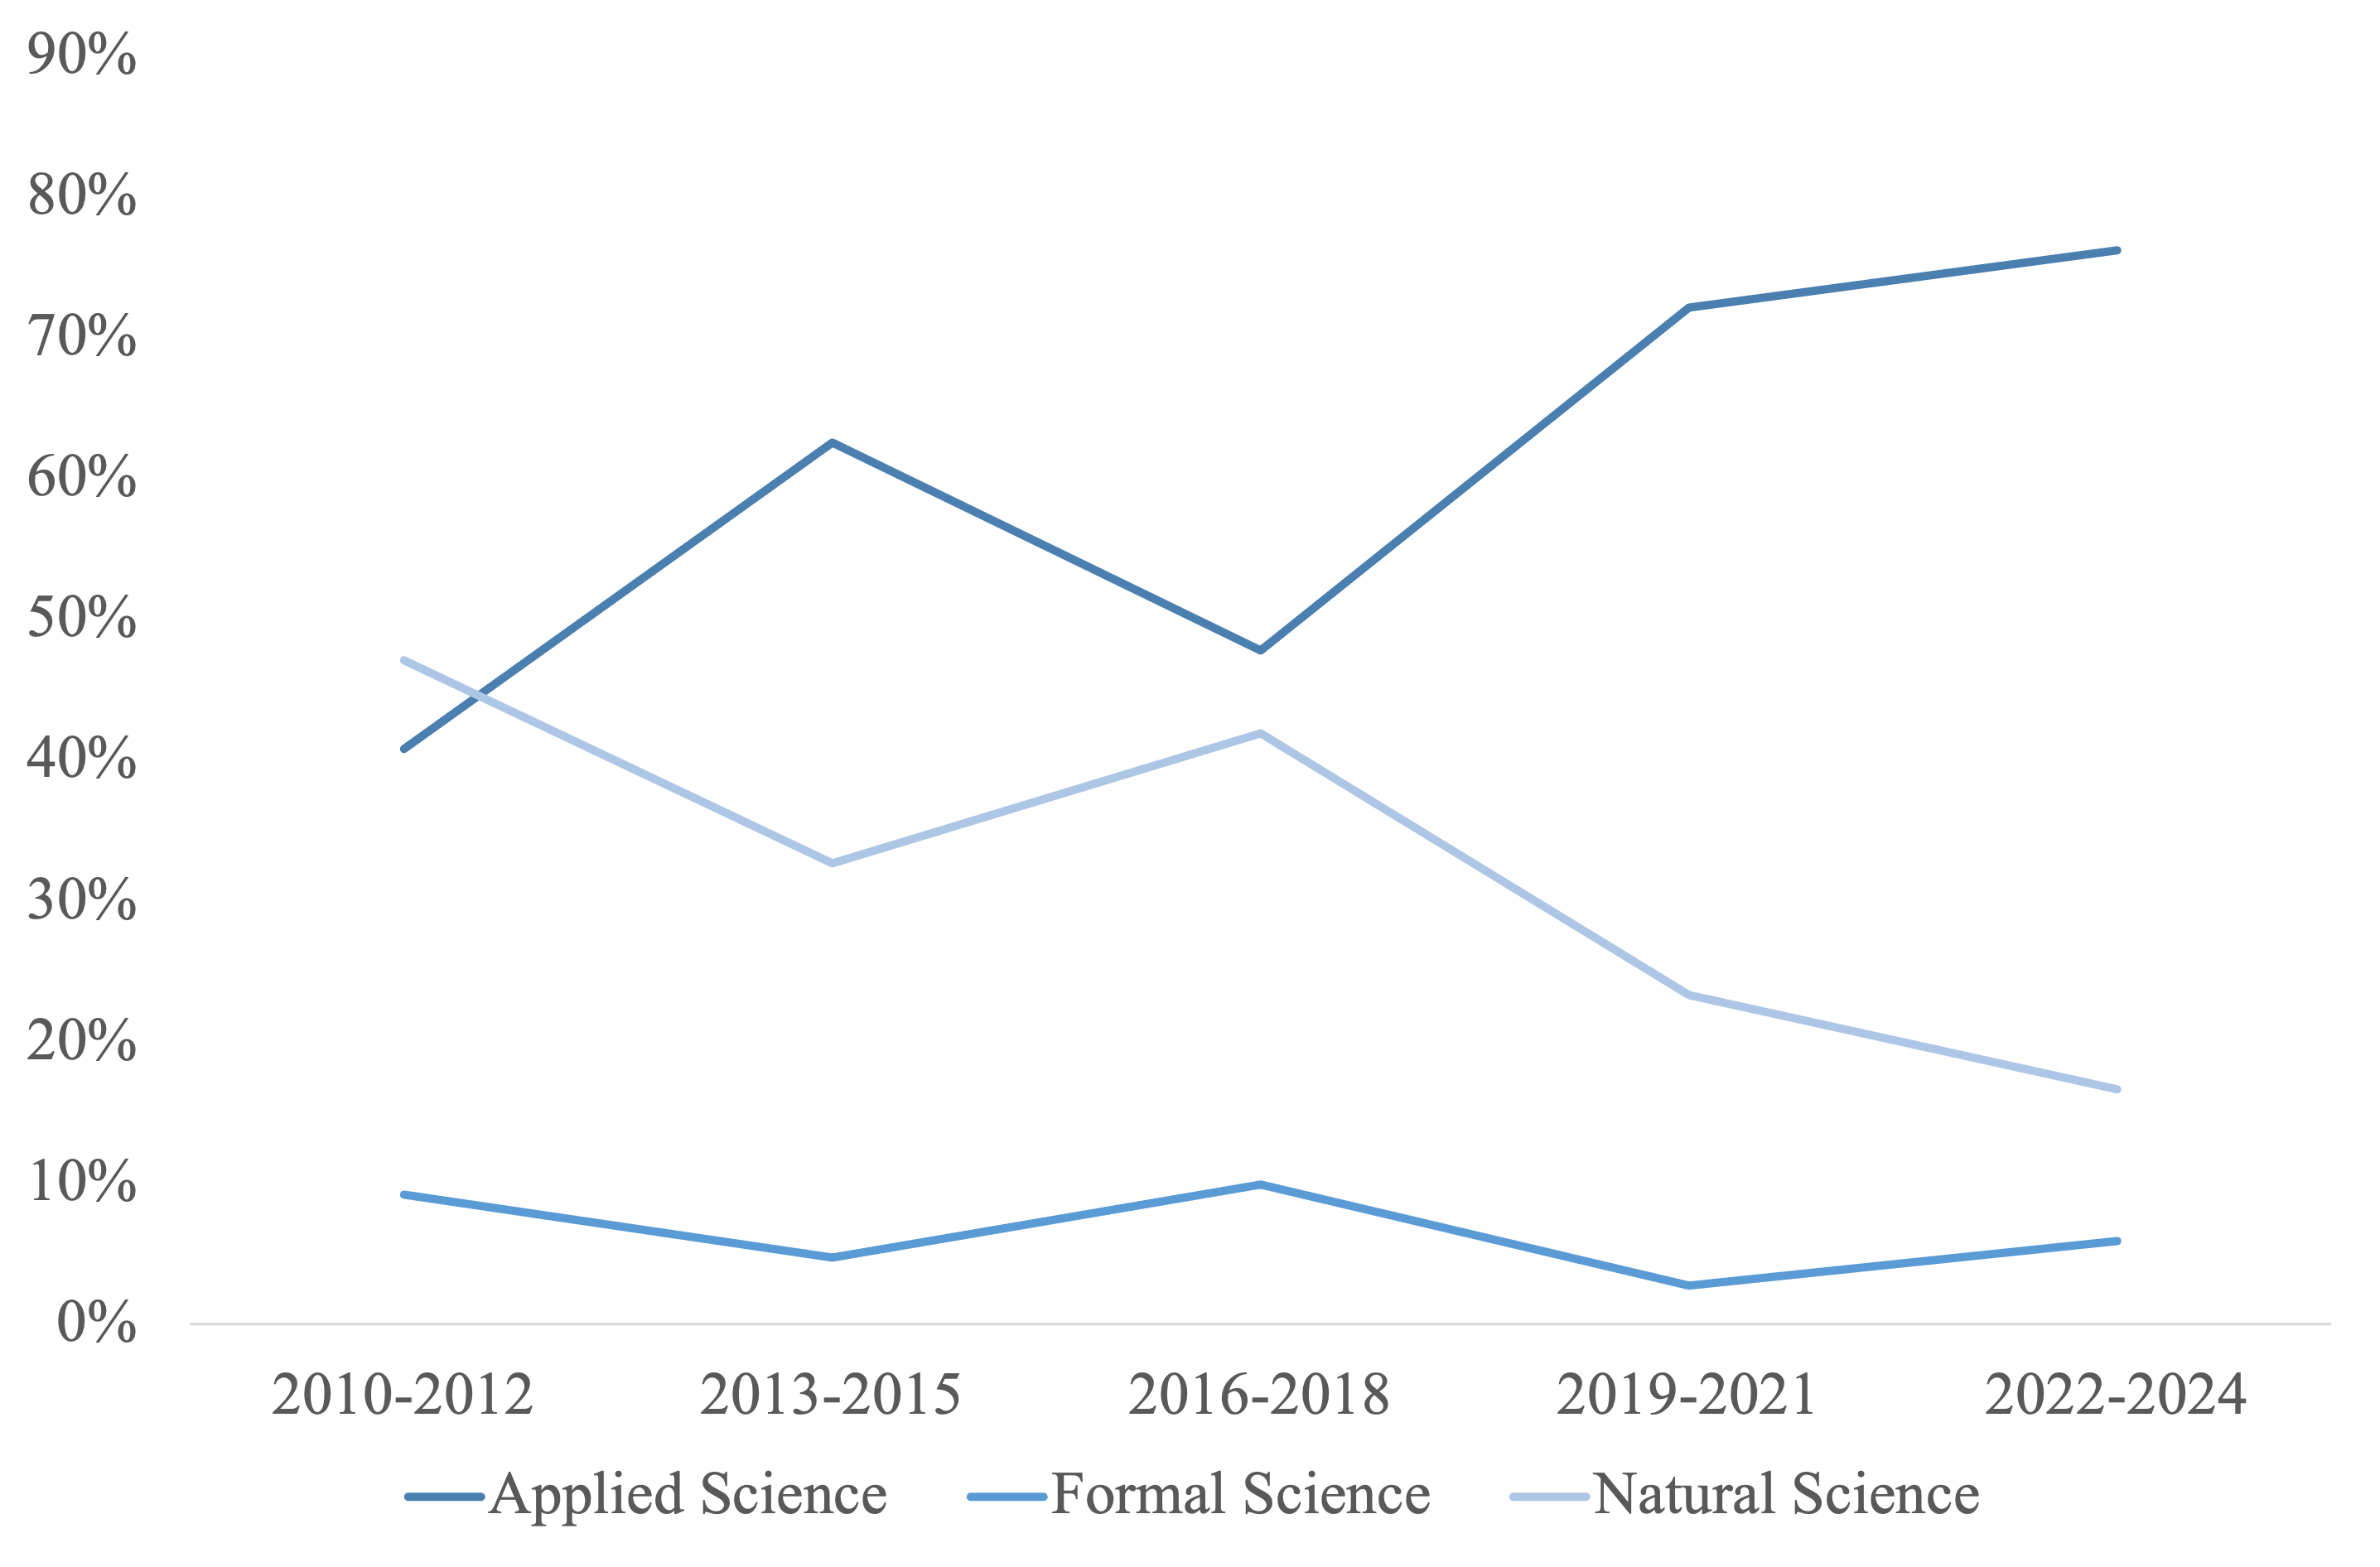
\includegraphics[width=\textwidth]{Figures/Evolution of Funding Distribution Across Categories.png}
       
    \end{minipage}
 
    \caption[Changing Subdomain Counts Across Categories Over Time]{
The upper figure showcases shifts in the count of funded subdomains within each category. The lower figure portrays the ratio of the number of funded subdomains normalized by the total project count.}
    \label{fig:combined}
\end{figure}
%TC:endignore
Despite minor fluctuations in the proportional distribution of project counts across various categories, a consistent trend emerges over the 21-year period. Applied Science and Natural Science have consistently maintained a notable advantage, collectively accounting for over half of the funded projects. Formal Science, particularly Mathematics and Statistics as foundational disciplines, have exhibited a consistent presence with a smaller yet stable number of funded projects. In contrast, Social Science received minimal funding during 2013-2015, rendering its contribution negligible and thus not represented on the line graph for visual clarity.\\


Funding for Applied Science projects shows an overall upward trend, whereas Natural Science projects exhibit an overall downward trend, and Formal Science projects maintain relatively stable funding allocation. Hence, it can be inferred that Applied Science has, to a certain extent, encroached upon the funding allocation that might have originally been directed toward Natural Science.\\

The number of subdomains within Applied Science and Natural Science has notably decreased, indicating a trend toward consolidation in both domains. I have created a heatmap for detailed analysis to gain more insight into these subdomain dynamics.\\

In comparison to the period between 2019 and 2021, a significant influx of funding in the realm of natural sciences has been directed toward environmental and material science from 2022 to 2024. However, no prominent research directions have been identified within applied science.
%TC:ignore
\begin{figure}[H]
    \centering
    \begin{minipage}{\textwidth}
        \centering
        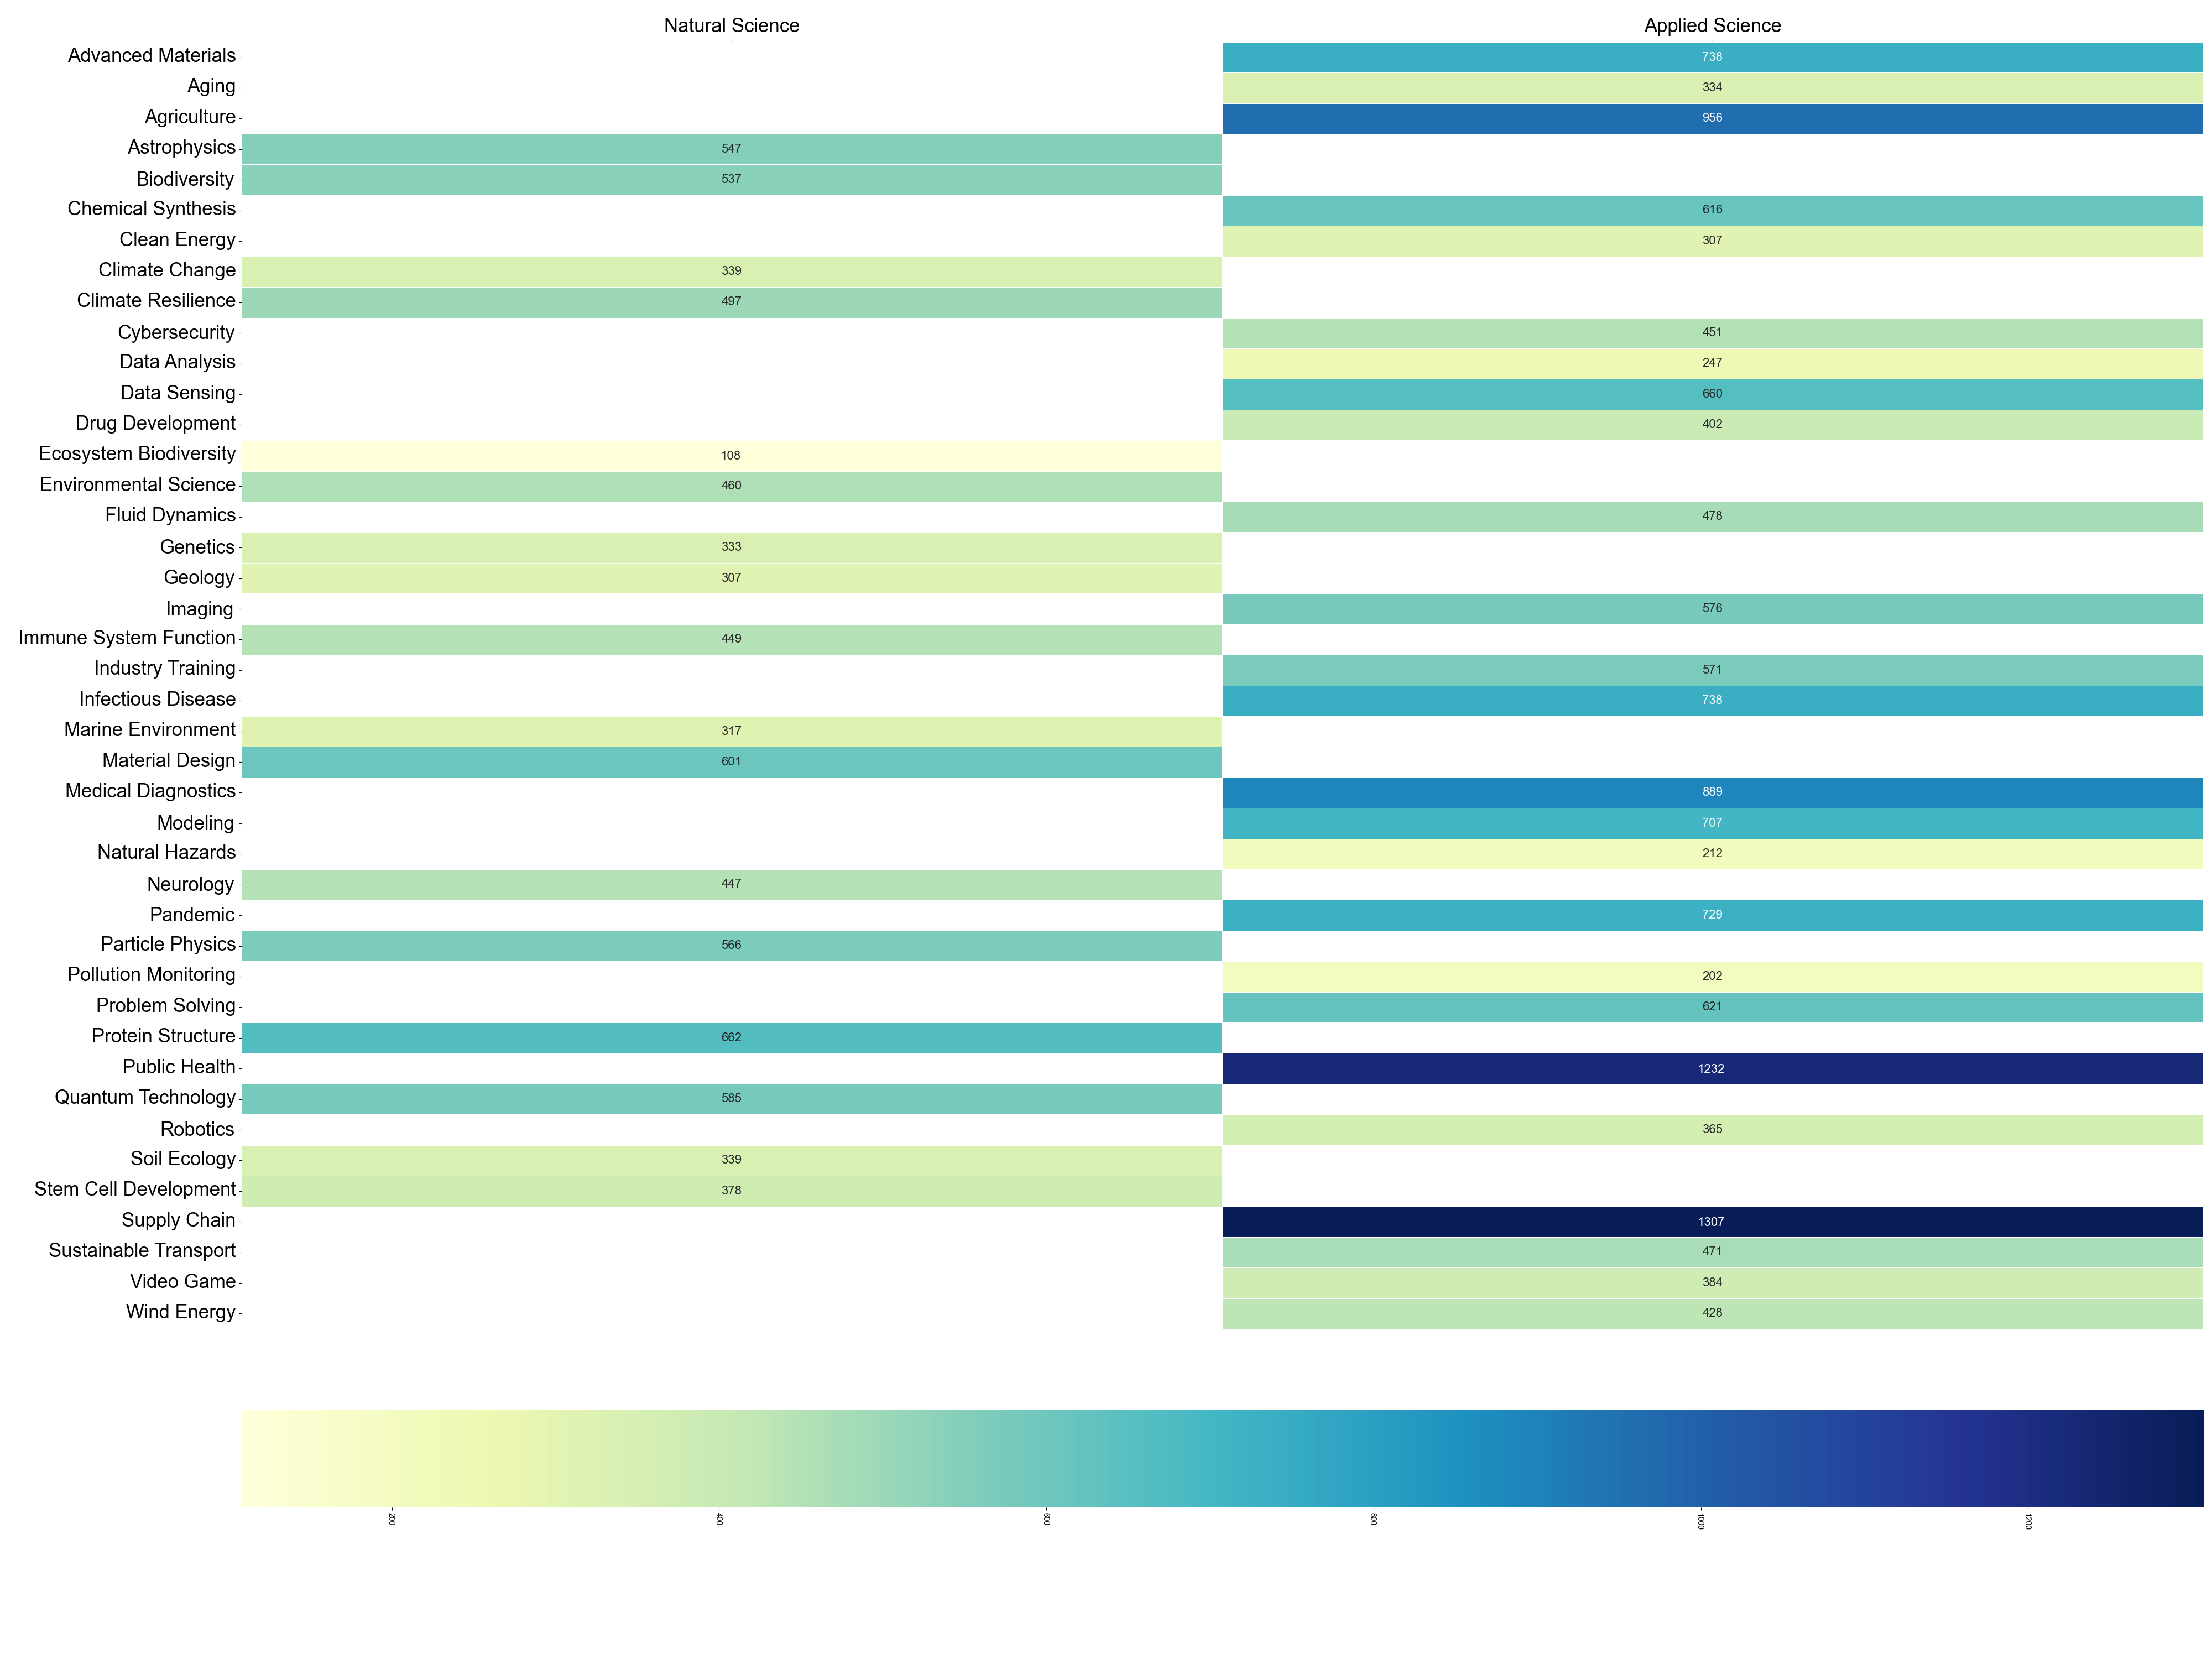
\includegraphics[width=0.95\textwidth]{ProjectReportTemplate/Figures/2019_2021_heatmap.png}
      
    \end{minipage}

    \begin{minipage}{\textwidth}
        \centering
        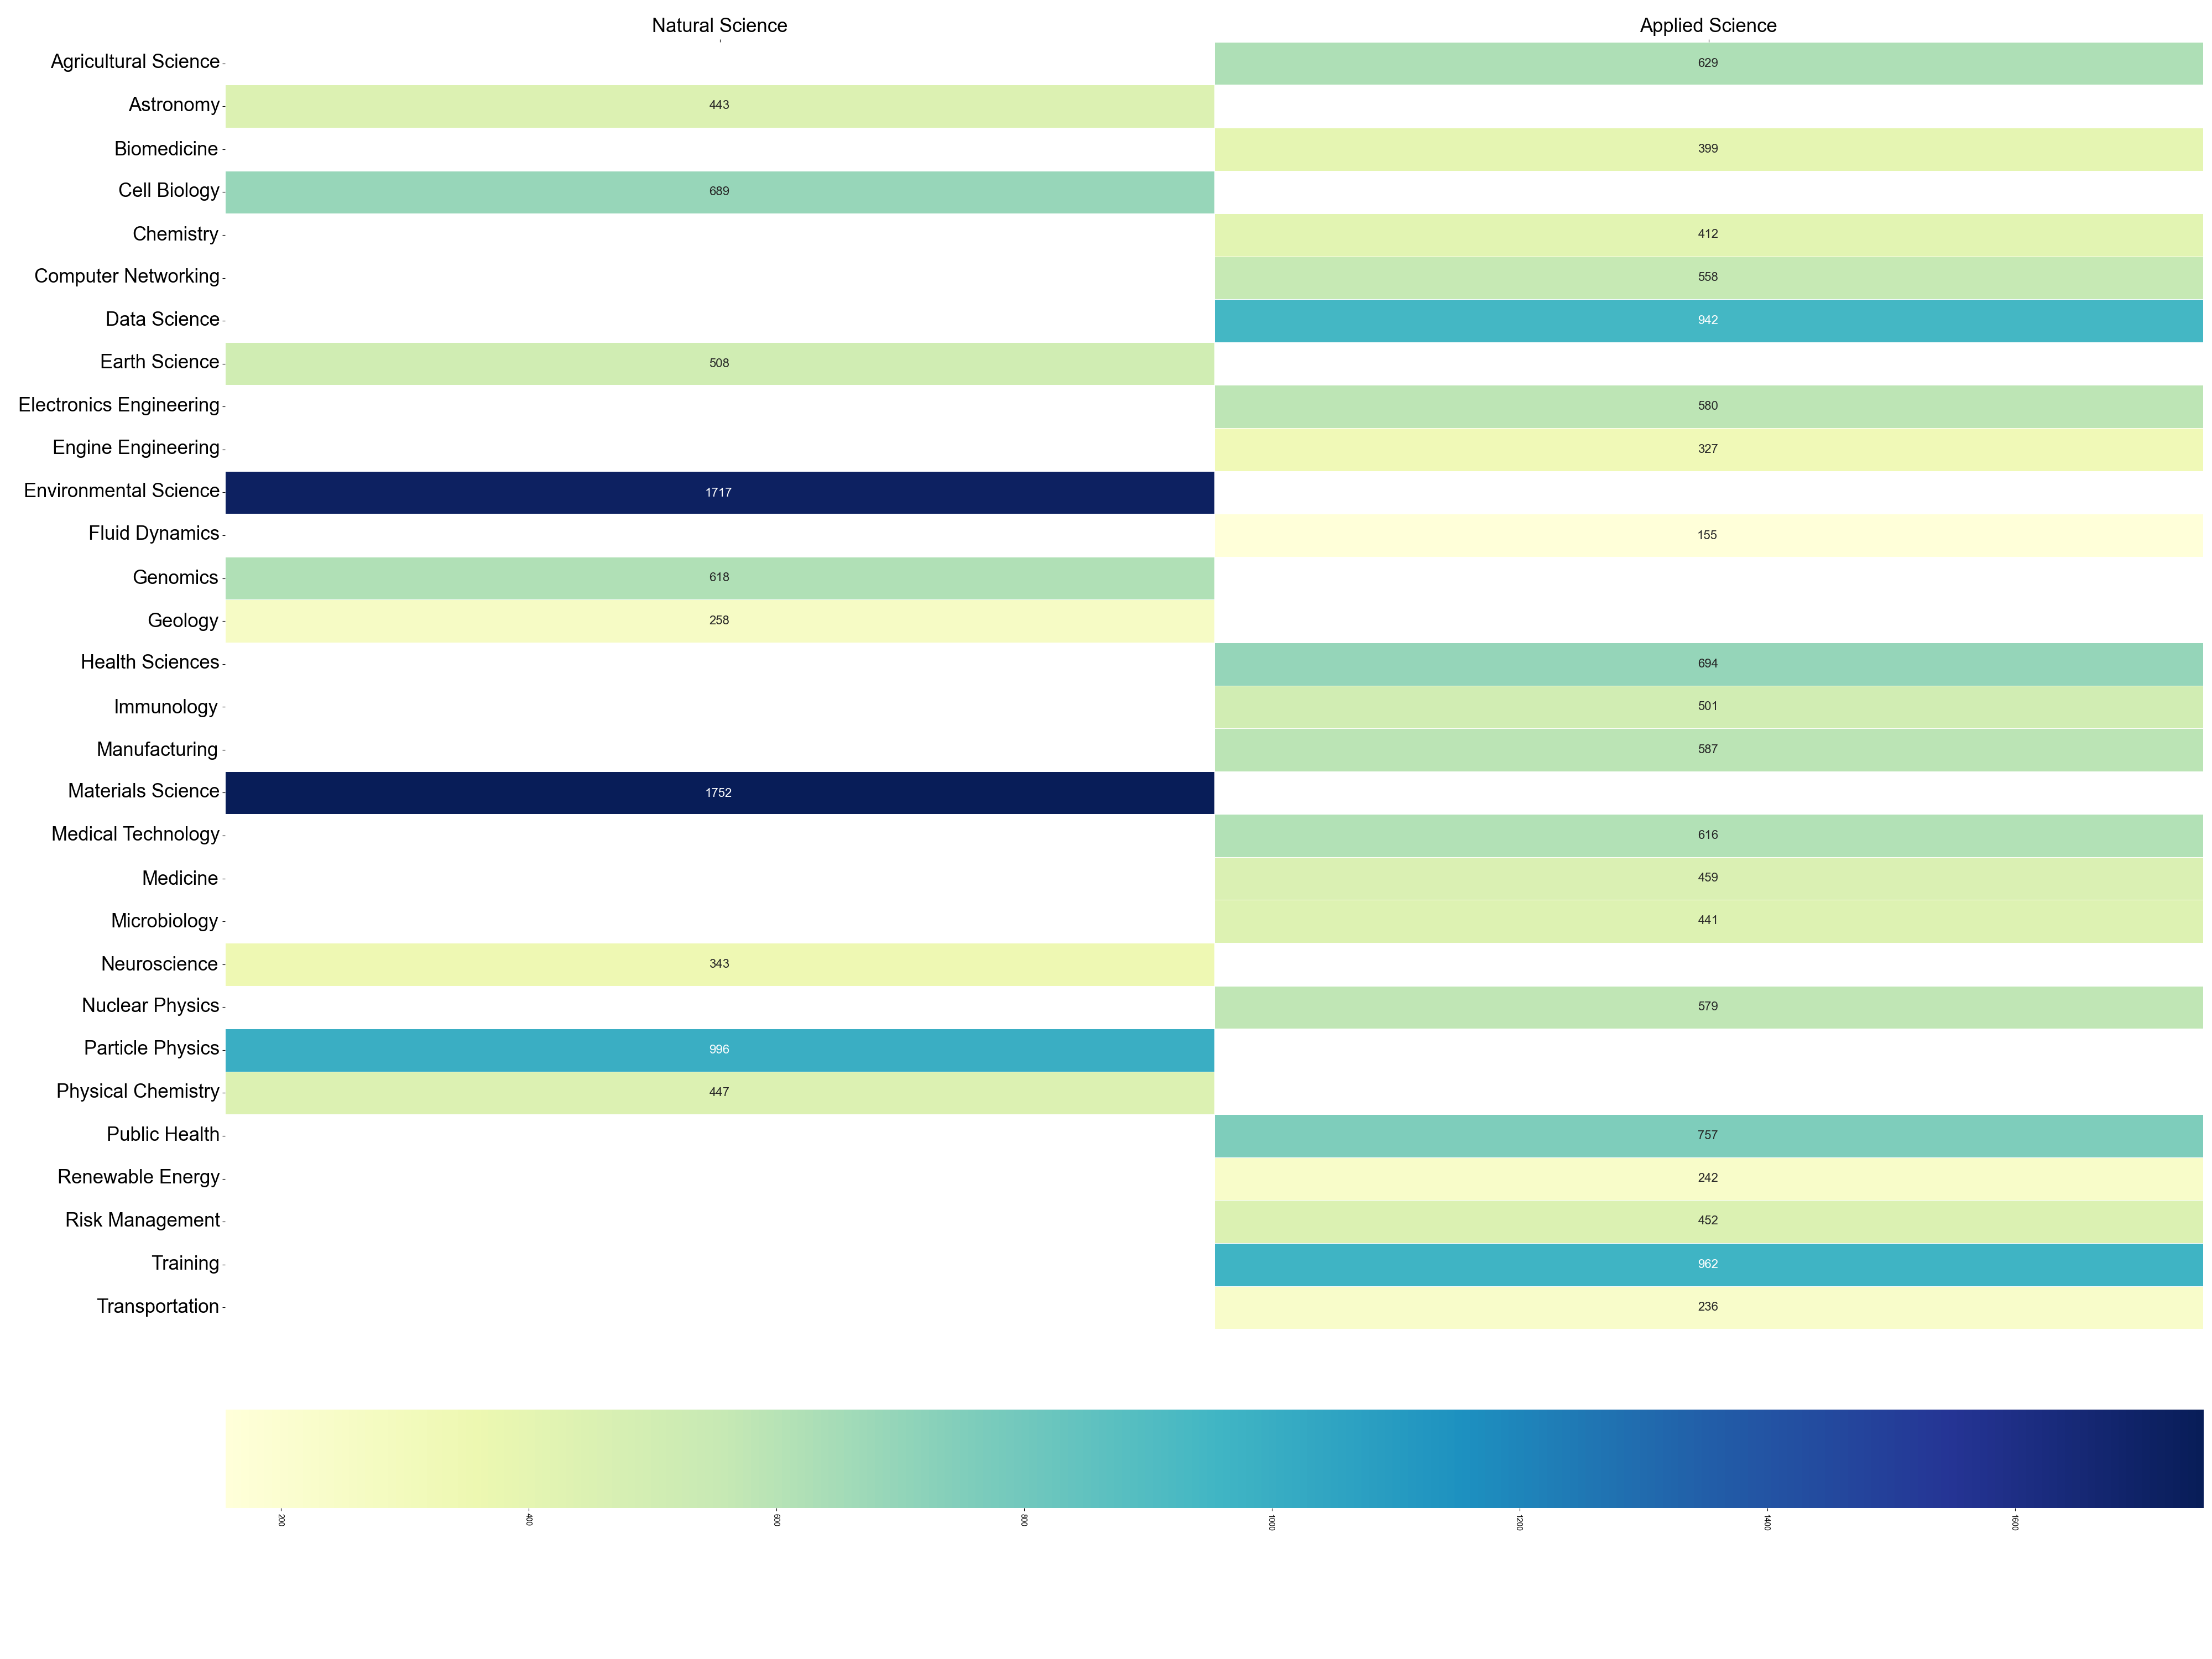
\includegraphics[width=0.95\textwidth]{ProjectReportTemplate/Figures/2022_2024_heatmap.png}
       
    \end{minipage}
 
    \caption[Project Counts distribution of Applied Science and Natural Science]{A huge amount of funding is directed towards Environmental Science and Materials Science.}
    \label{fig:combined}
\end{figure}
%TC:endignore


An aspect worthy of attention is the sustained inclusion of ecology within the funded projects list, maintaining a prominent position throughout each three-year interval. 
%TC:ignore
\begin{figure}[H]
\centering
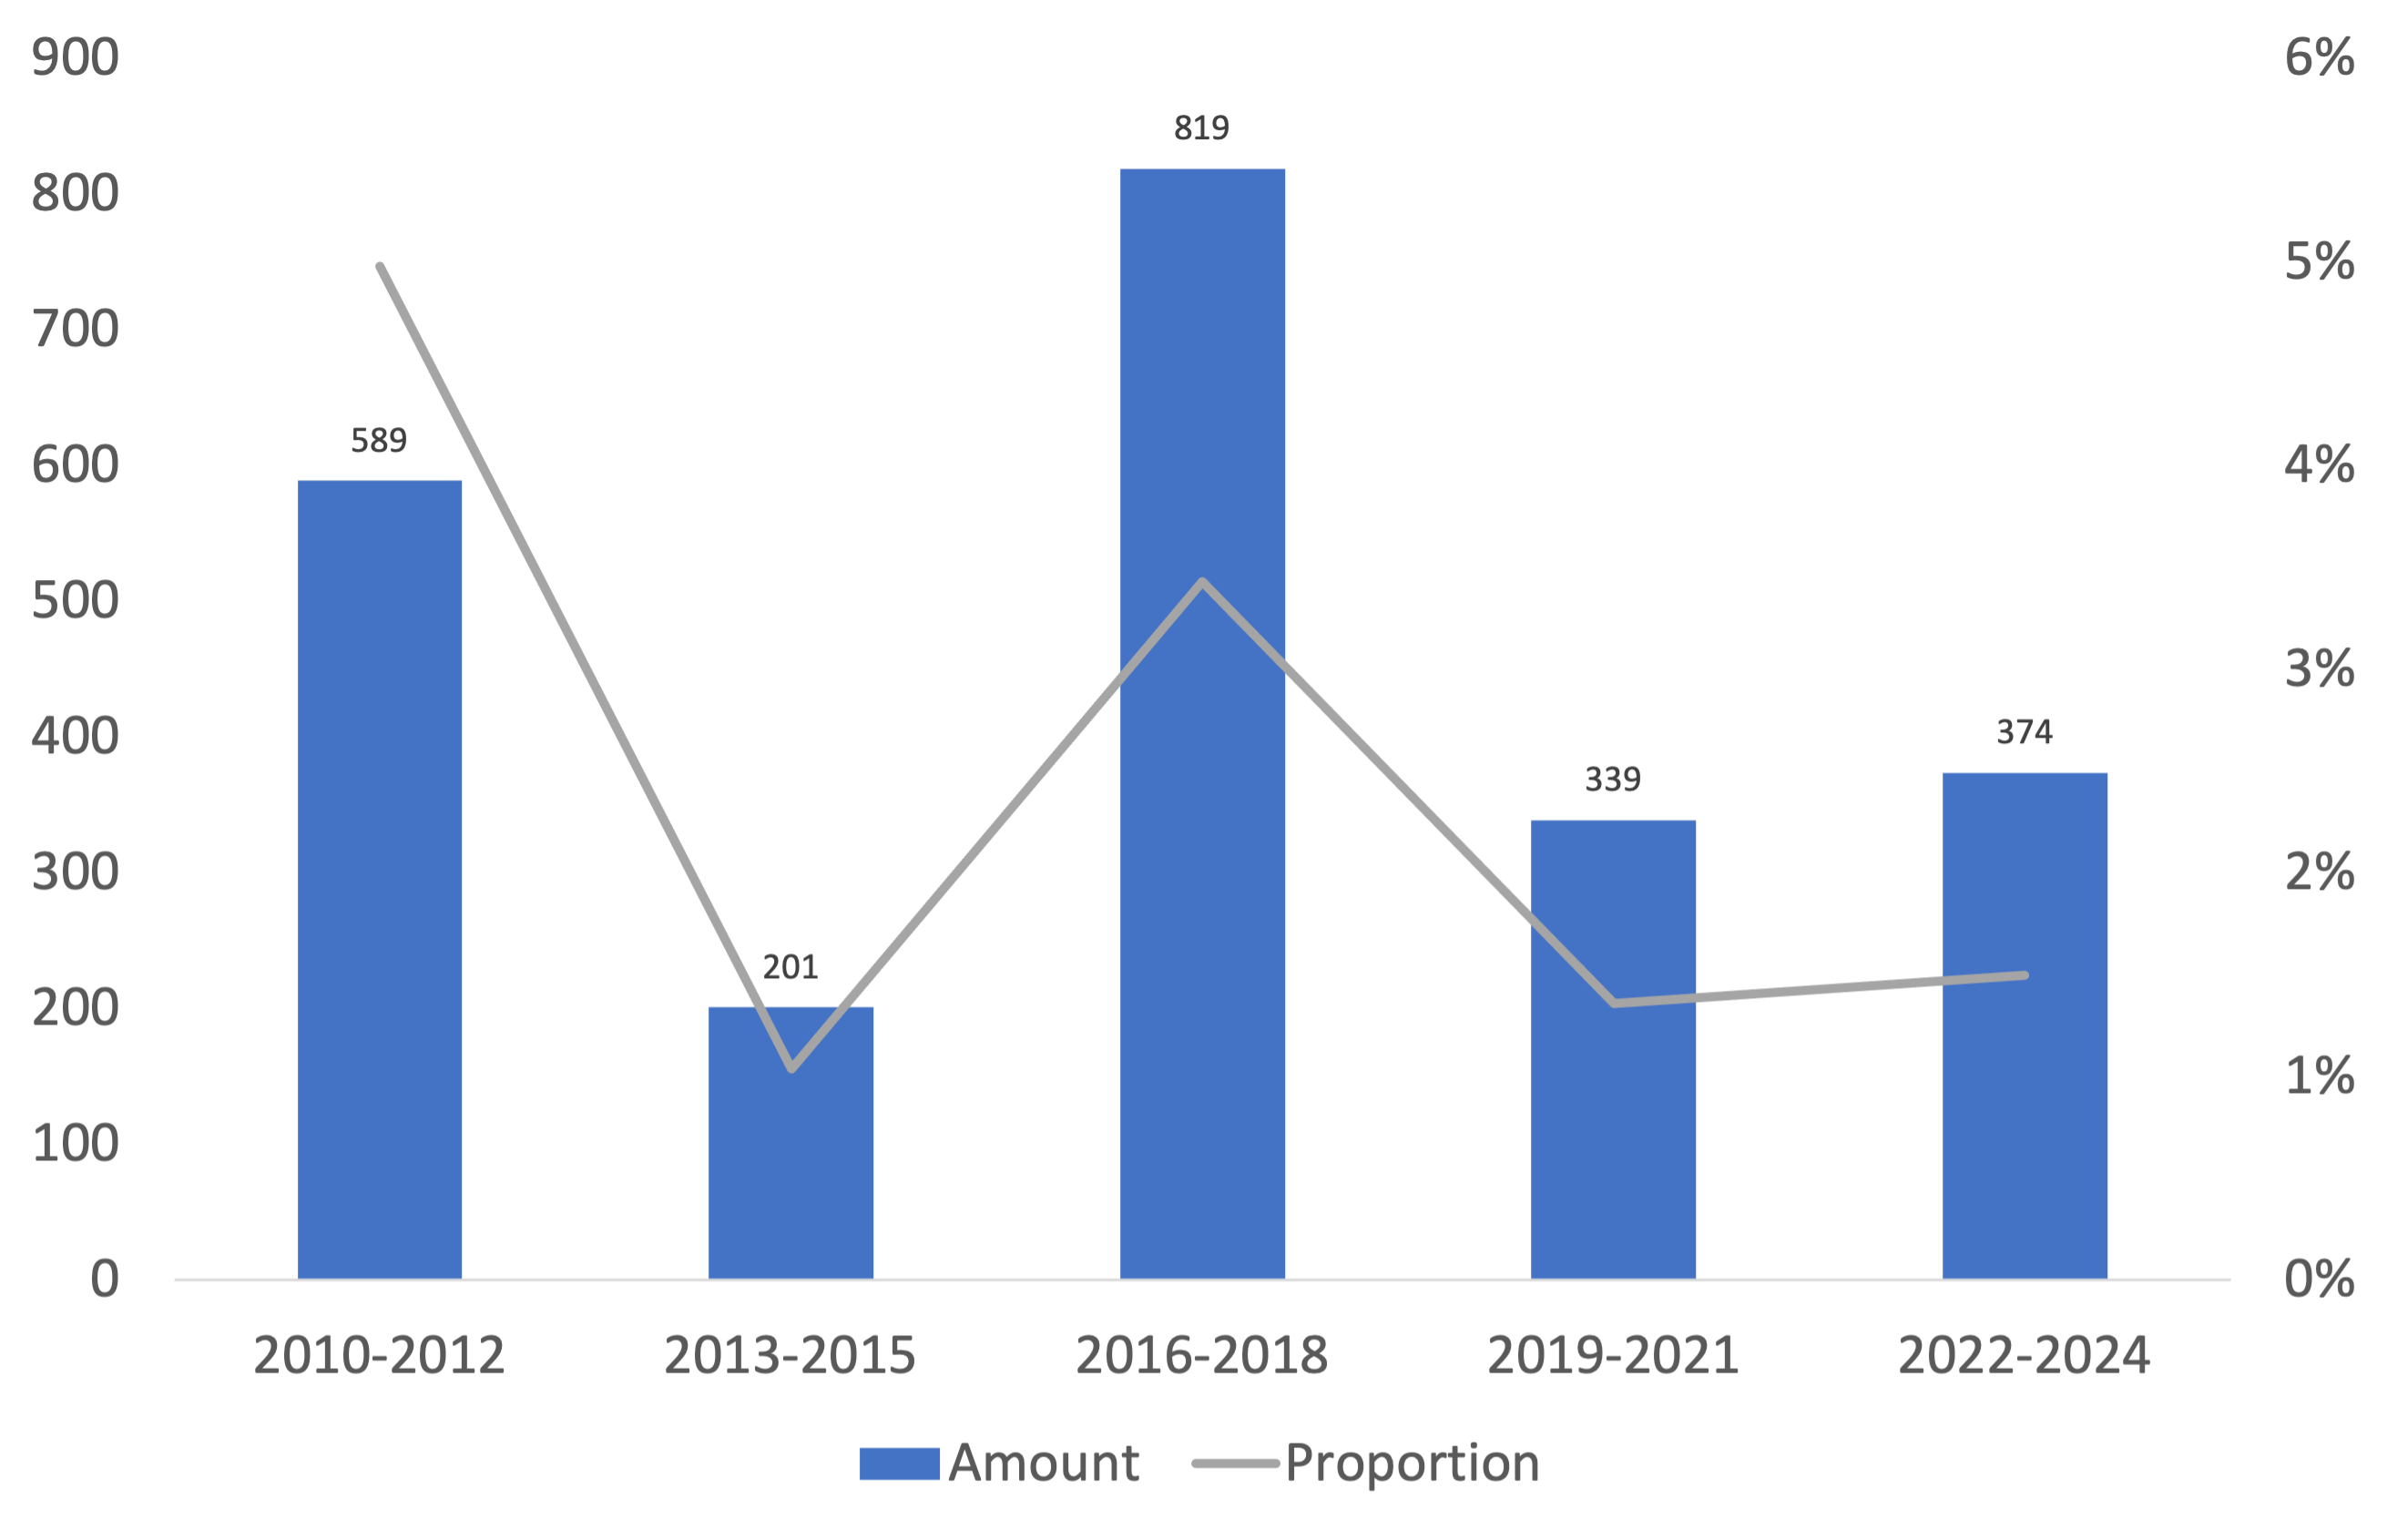
\includegraphics[scale=0.7]{Figures/Landscape of Ecology Funding.png}
\caption[Changing Landscape of Ecology Funding]{Ecology has consistently secured funding for several hundred projects during each triennial period.}
\label{figure} 
\end{figure}
%TC:endignore
In contrast, evolutionary biology has not received funding at a high frequency, with only 203 projects receiving funding between 2010 and 2012. Subsequently, the number of funded projects related to this field has remained notably low across the entire dataset.

\section*{Overall Analysis Based on Funding Amount}

In addition to project count, the amount of funding allocated to projects in different domains can also indicate the level of attention and popularity within each respective field. The funding received by projects across various domains reflects the extent of emphasis and interest dedicated to those domains, thereby providing valuable insights into their prominence and significance.\\

Over the past two decades, there has been a noticeable upward trend in the funding amounts provided by UKRI. Specifically, the funding amounts for the periods 2010-2012, 2013-2015, 2016-2018, 2019-2021, and 2022-2024 have been £3,150,014,803, £5,859,873,507, £7,314,254,625, £7,507,960,726, and £7,285,275,813, respectively. It is important to emphasize that the funding amount for 2022-2024 is based on data up to 2022 rather than being the most up-to-date information. Consequently, a substantial number of projects have not yet been included in the analyzed data, resulting in a seemingly reduced figure. Furthermore, numerous projects are still in the application phase, including cases like the "Knowledge transfer partnerships (KTP): 2023 to 2024 round four," where the allocation of the £9,000,000 funding remains pending.\\


UKRI continues to invest more in "applied science" and "natural science." While the proportions of these two categories of projects have changed over time, their combined total has consistently remained above 80\%. Notably, during 2013-2015 and 2016-2018, this proportion reached an astonishing 96\%. This trend highlights the significant importance UKRI places on these areas and underscores the greater need for research funding for projects within these domains. It also indicates that, to a certain extent, they have reallocated funding from other category projects.\\

%TC:ignore
\begin{figure}[H]
\centering
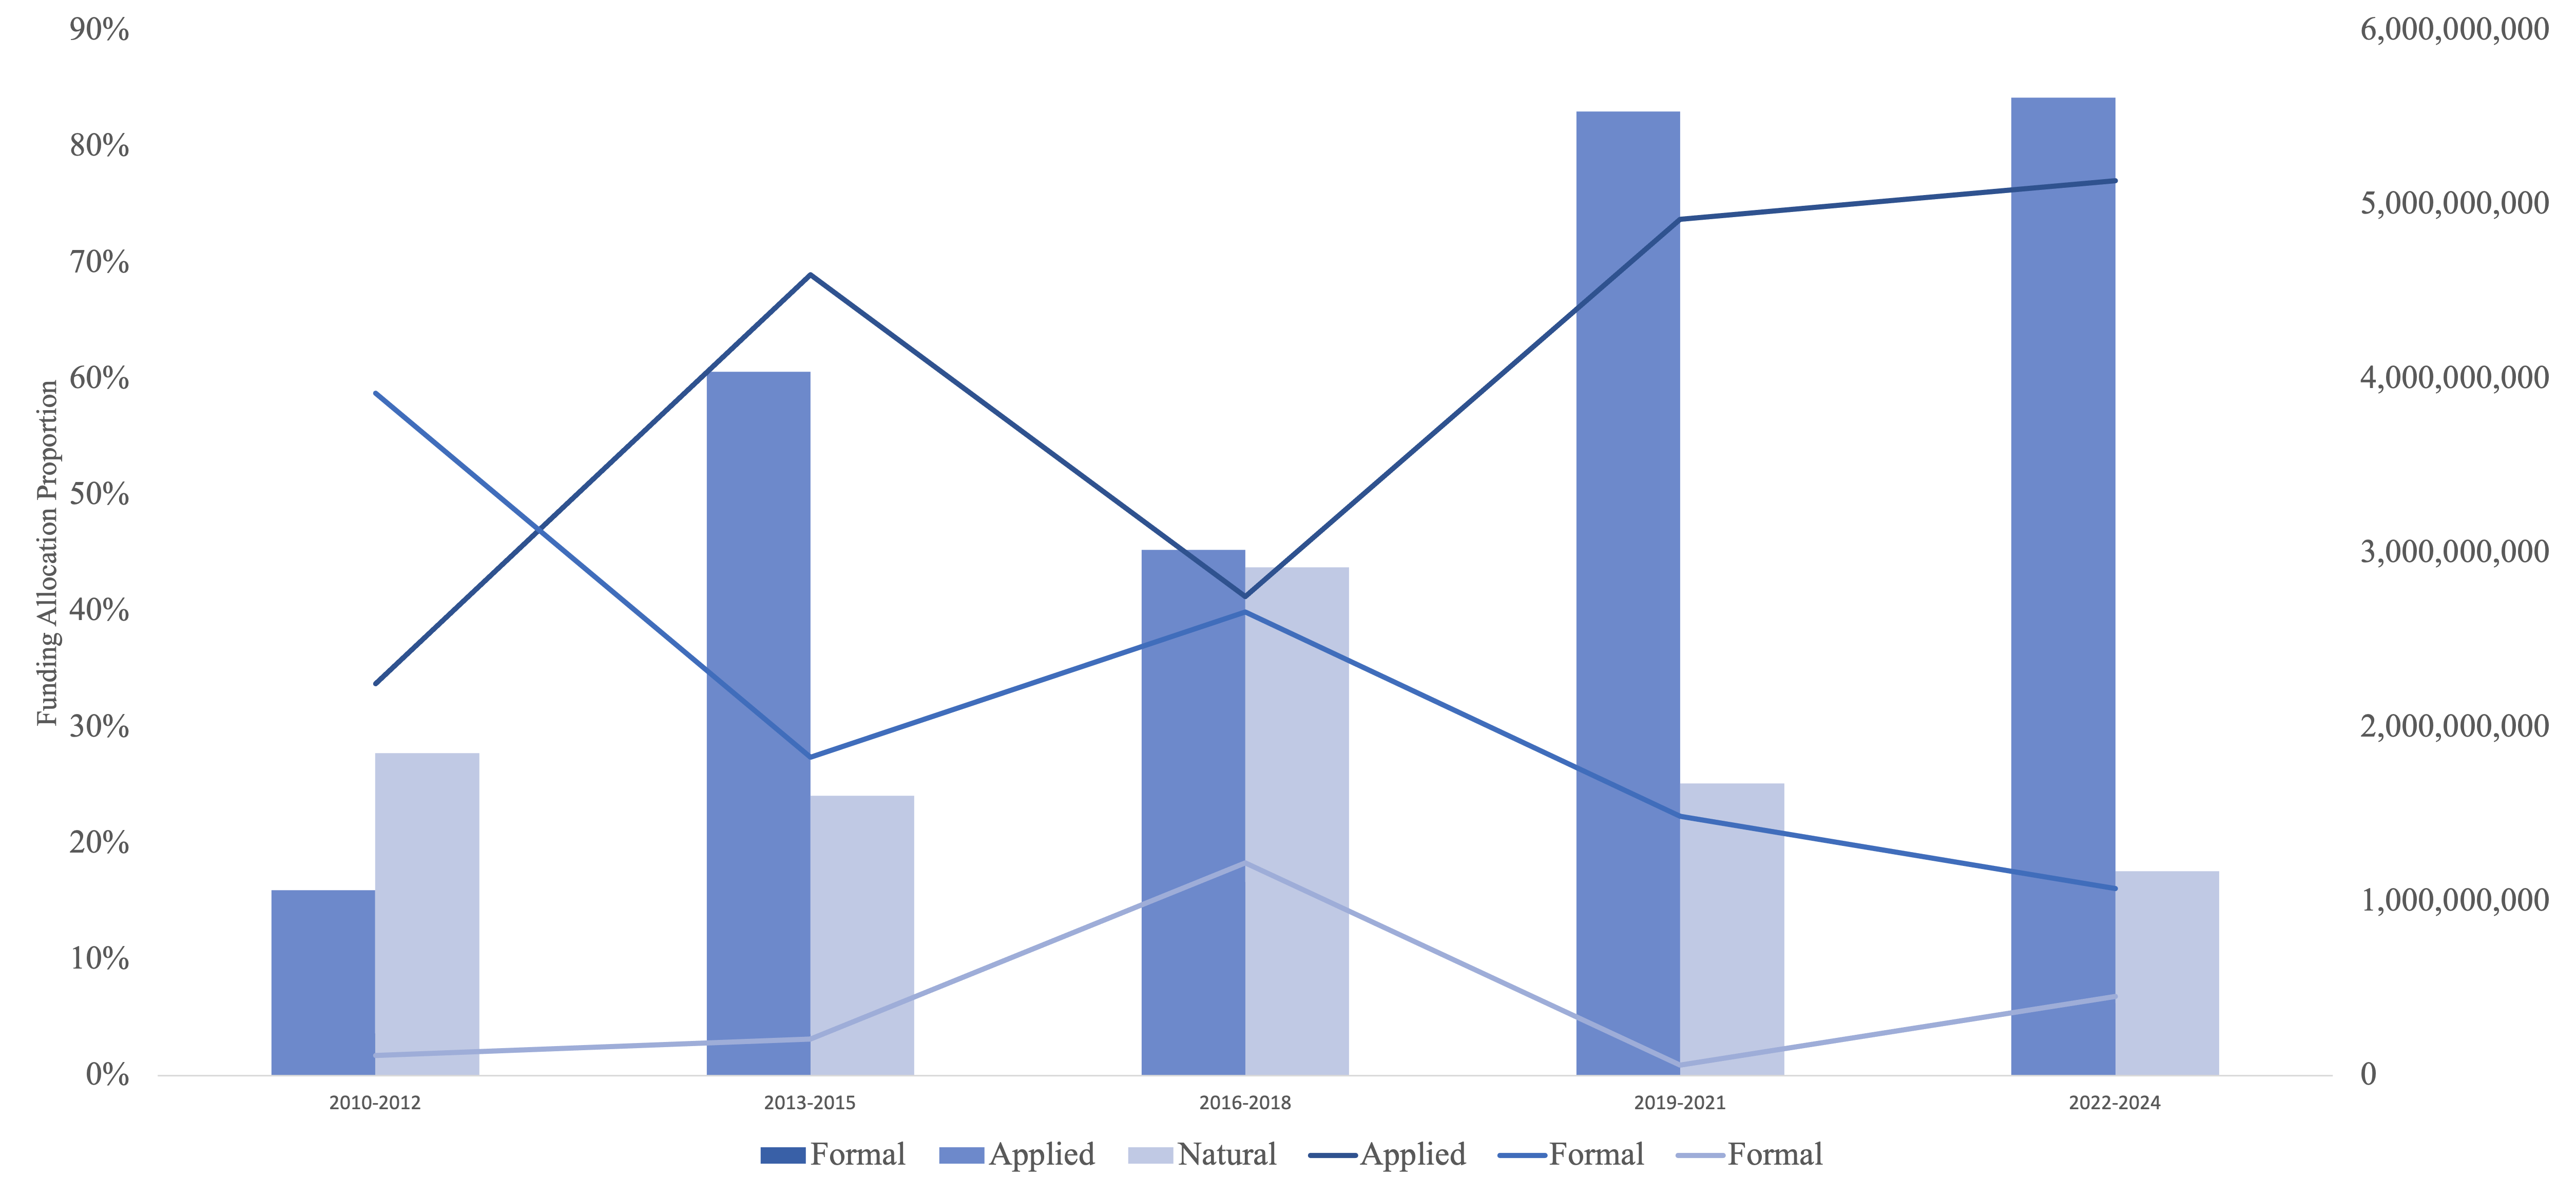
\includegraphics[scale=0.4]{Figures/funding_amount.png}
\caption[Evolution of Funding Trends Across Categories]{Applied Science continues to exhibit an upward trajectory in funding amounts, maintaining the highest proportion of funding allocation.}
\label{figure3.5} 
\end{figure}
%TC:endignore
Upon closer examination of each three-year interval, in each interval, UKRI's focus within the natural sciences field has continuously evolved. For instance, From 2013 to 2015, UKRI allocated substantial funding towards Energy Systems and Technology Innovation, providing support amounting to £512,227,820 and £406,407,200, respectively. However, of even greater significance is UKRI's evident keenness towards the health and longevity of humanity. Cell Biology received a substantial grant of £48,791,642, while Aging research secured £310,492,126, and Public Health initiatives were granted £185,898,579. Further, considerable support was extended to Medical Technology with £83,056,741 in funding, and Cardiovascular Diseases research obtained £65,710,644, among numerous other related projects. This demonstrates UKRI's concerted efforts to drive advancements in diverse fields critical to human well-being.\\

However, a notable shift in focus occurred during 2016-2018, as UKRI redirected its attention towards environmental concerns. During this period, natural science topics that received the highest funding included Energy Systems with £112,236,139 and Environmental Pollution with £358,116,908, encompassing Earth Science with a funding allocation of £163,914,390. This phase witnessed a substantial increase in funding for numerous environmental protection and sustainability initiatives. Similarly, in the subsequent interval of 2019-2021, UKRI continued this trend by allocating £127,302,749 to Wind Energy, £94,358,531 to Clean Energy, and a substantial £155,449,671 to Marine Environment projects.\\


%TC:ignore
\begin{figure}[H]
    \centering

    \begin{subfigure}{\textwidth}
        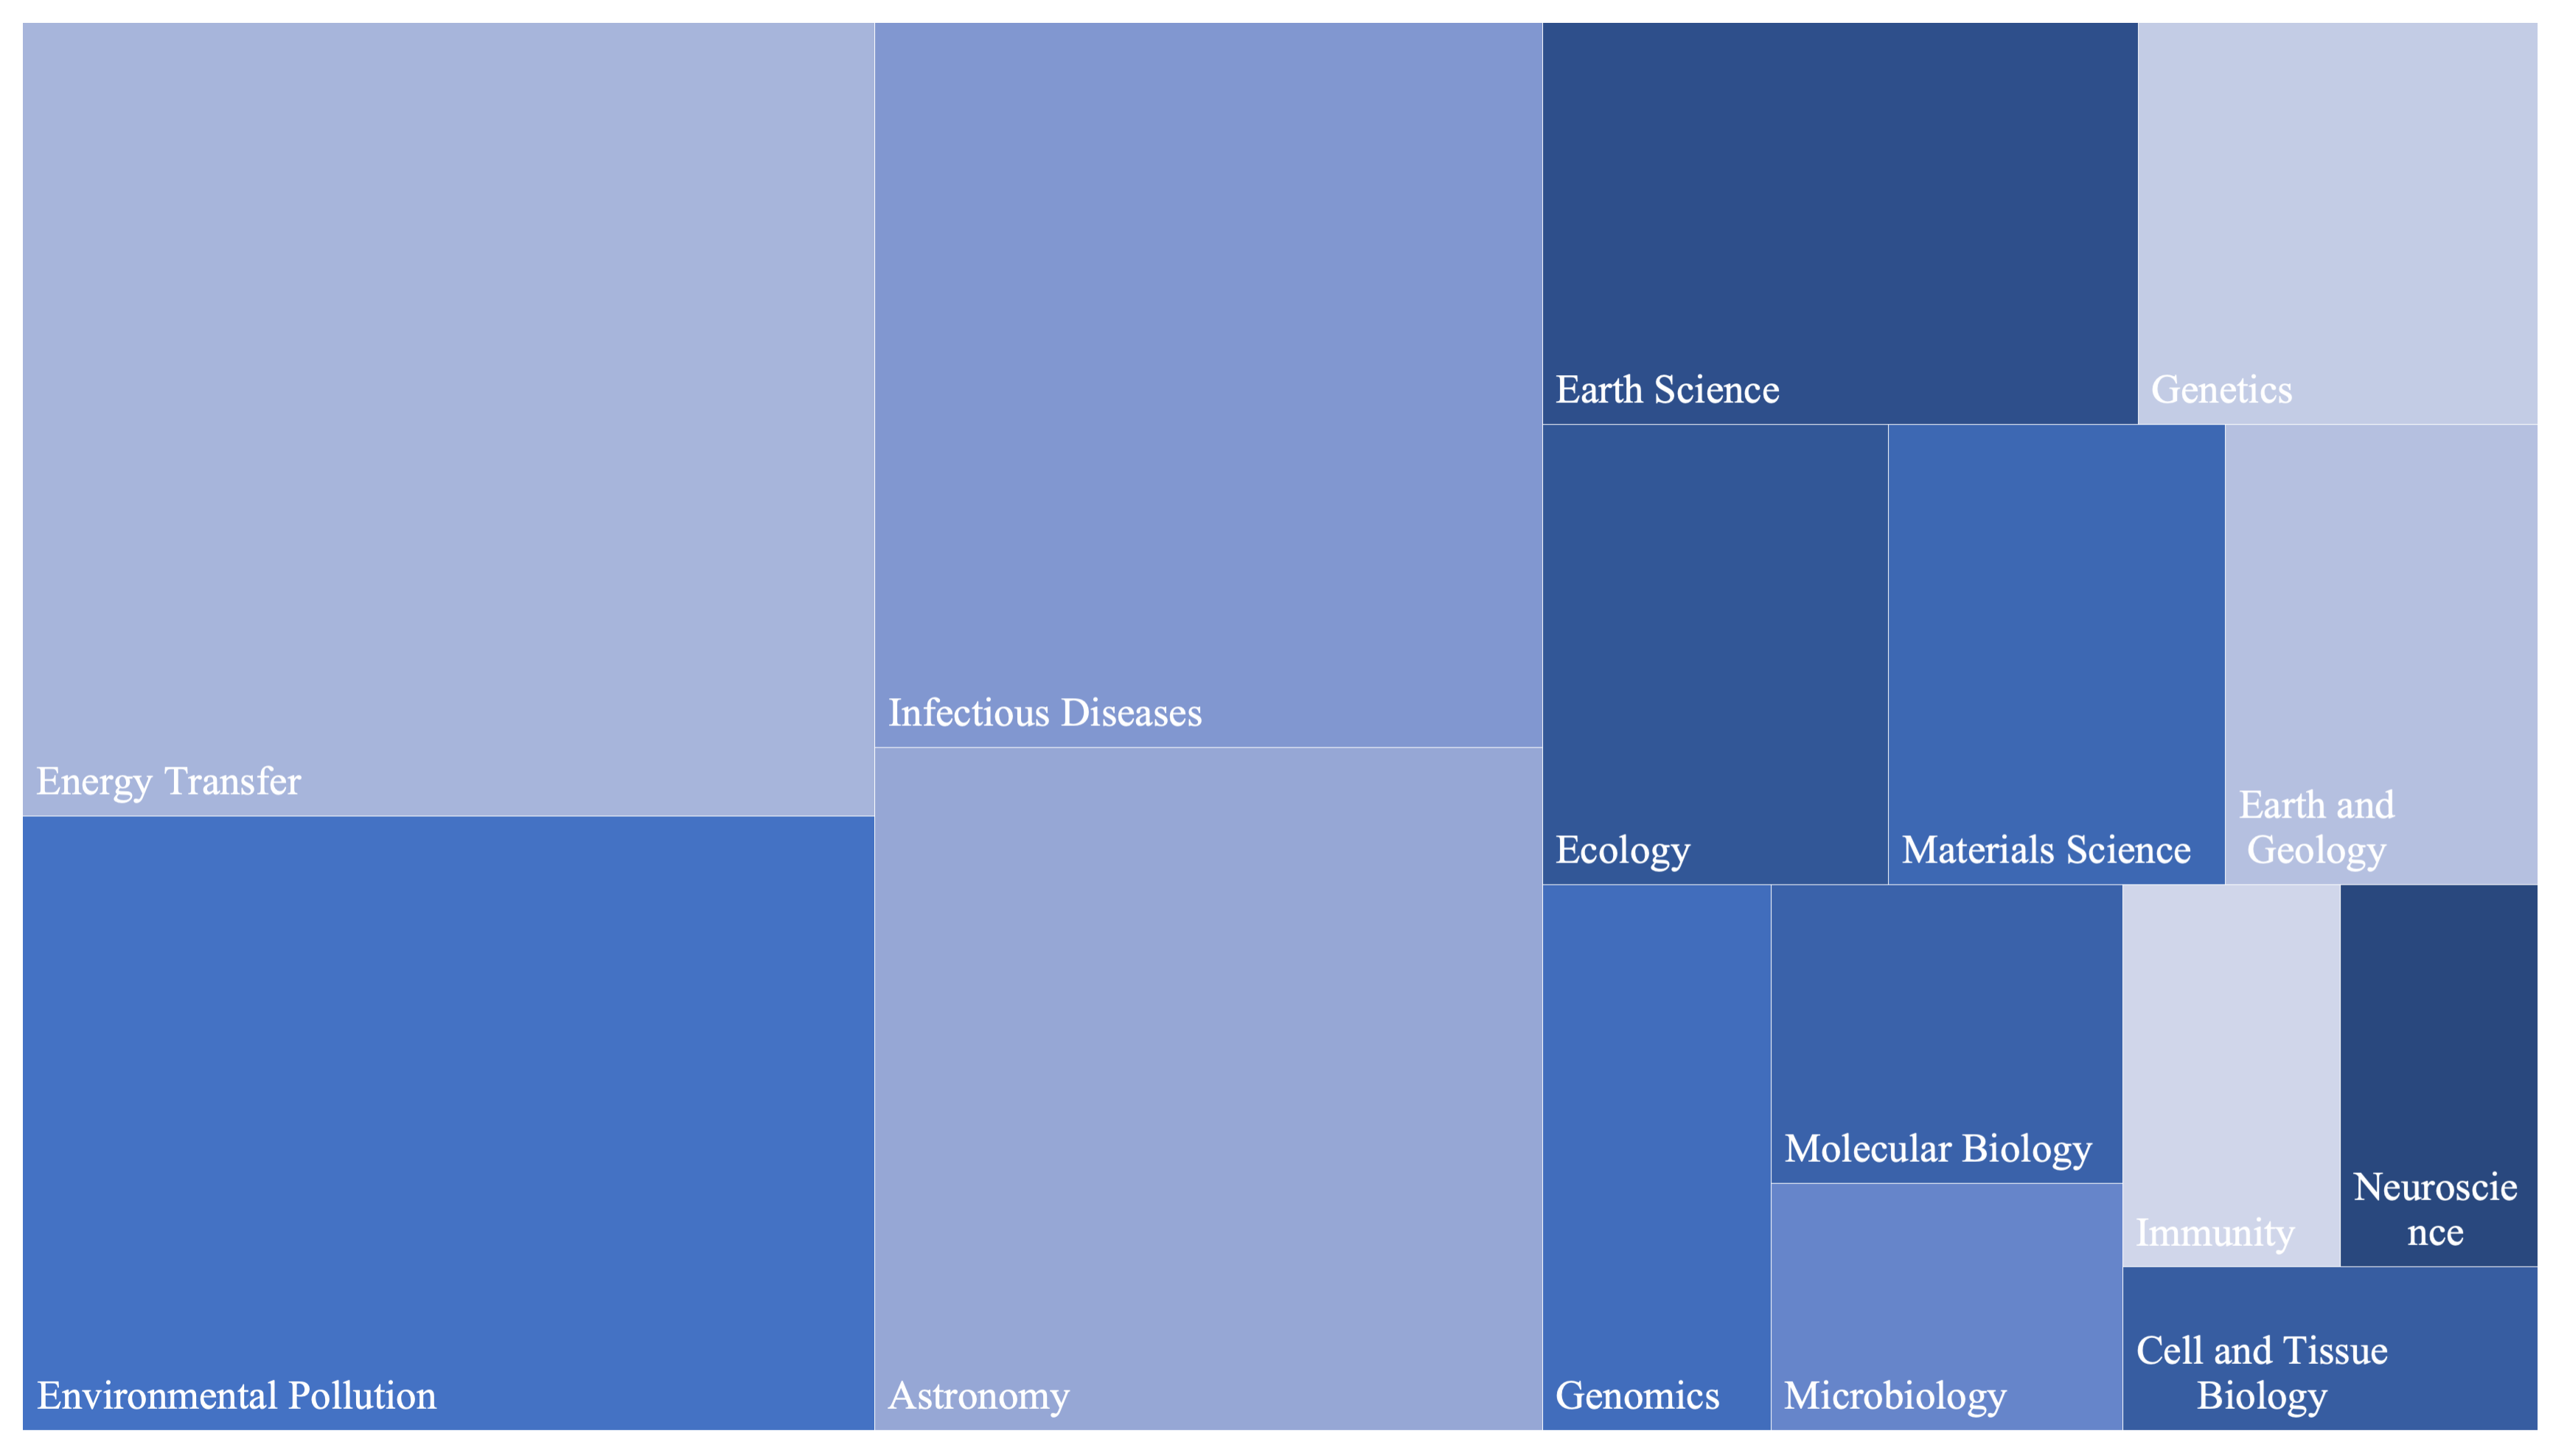
\includegraphics[width=\textwidth]{Figures/Overview of Natural Science Projects Funded in 2016-2018.png}

    \end{subfigure}
    \begin{subfigure}{\textwidth}
        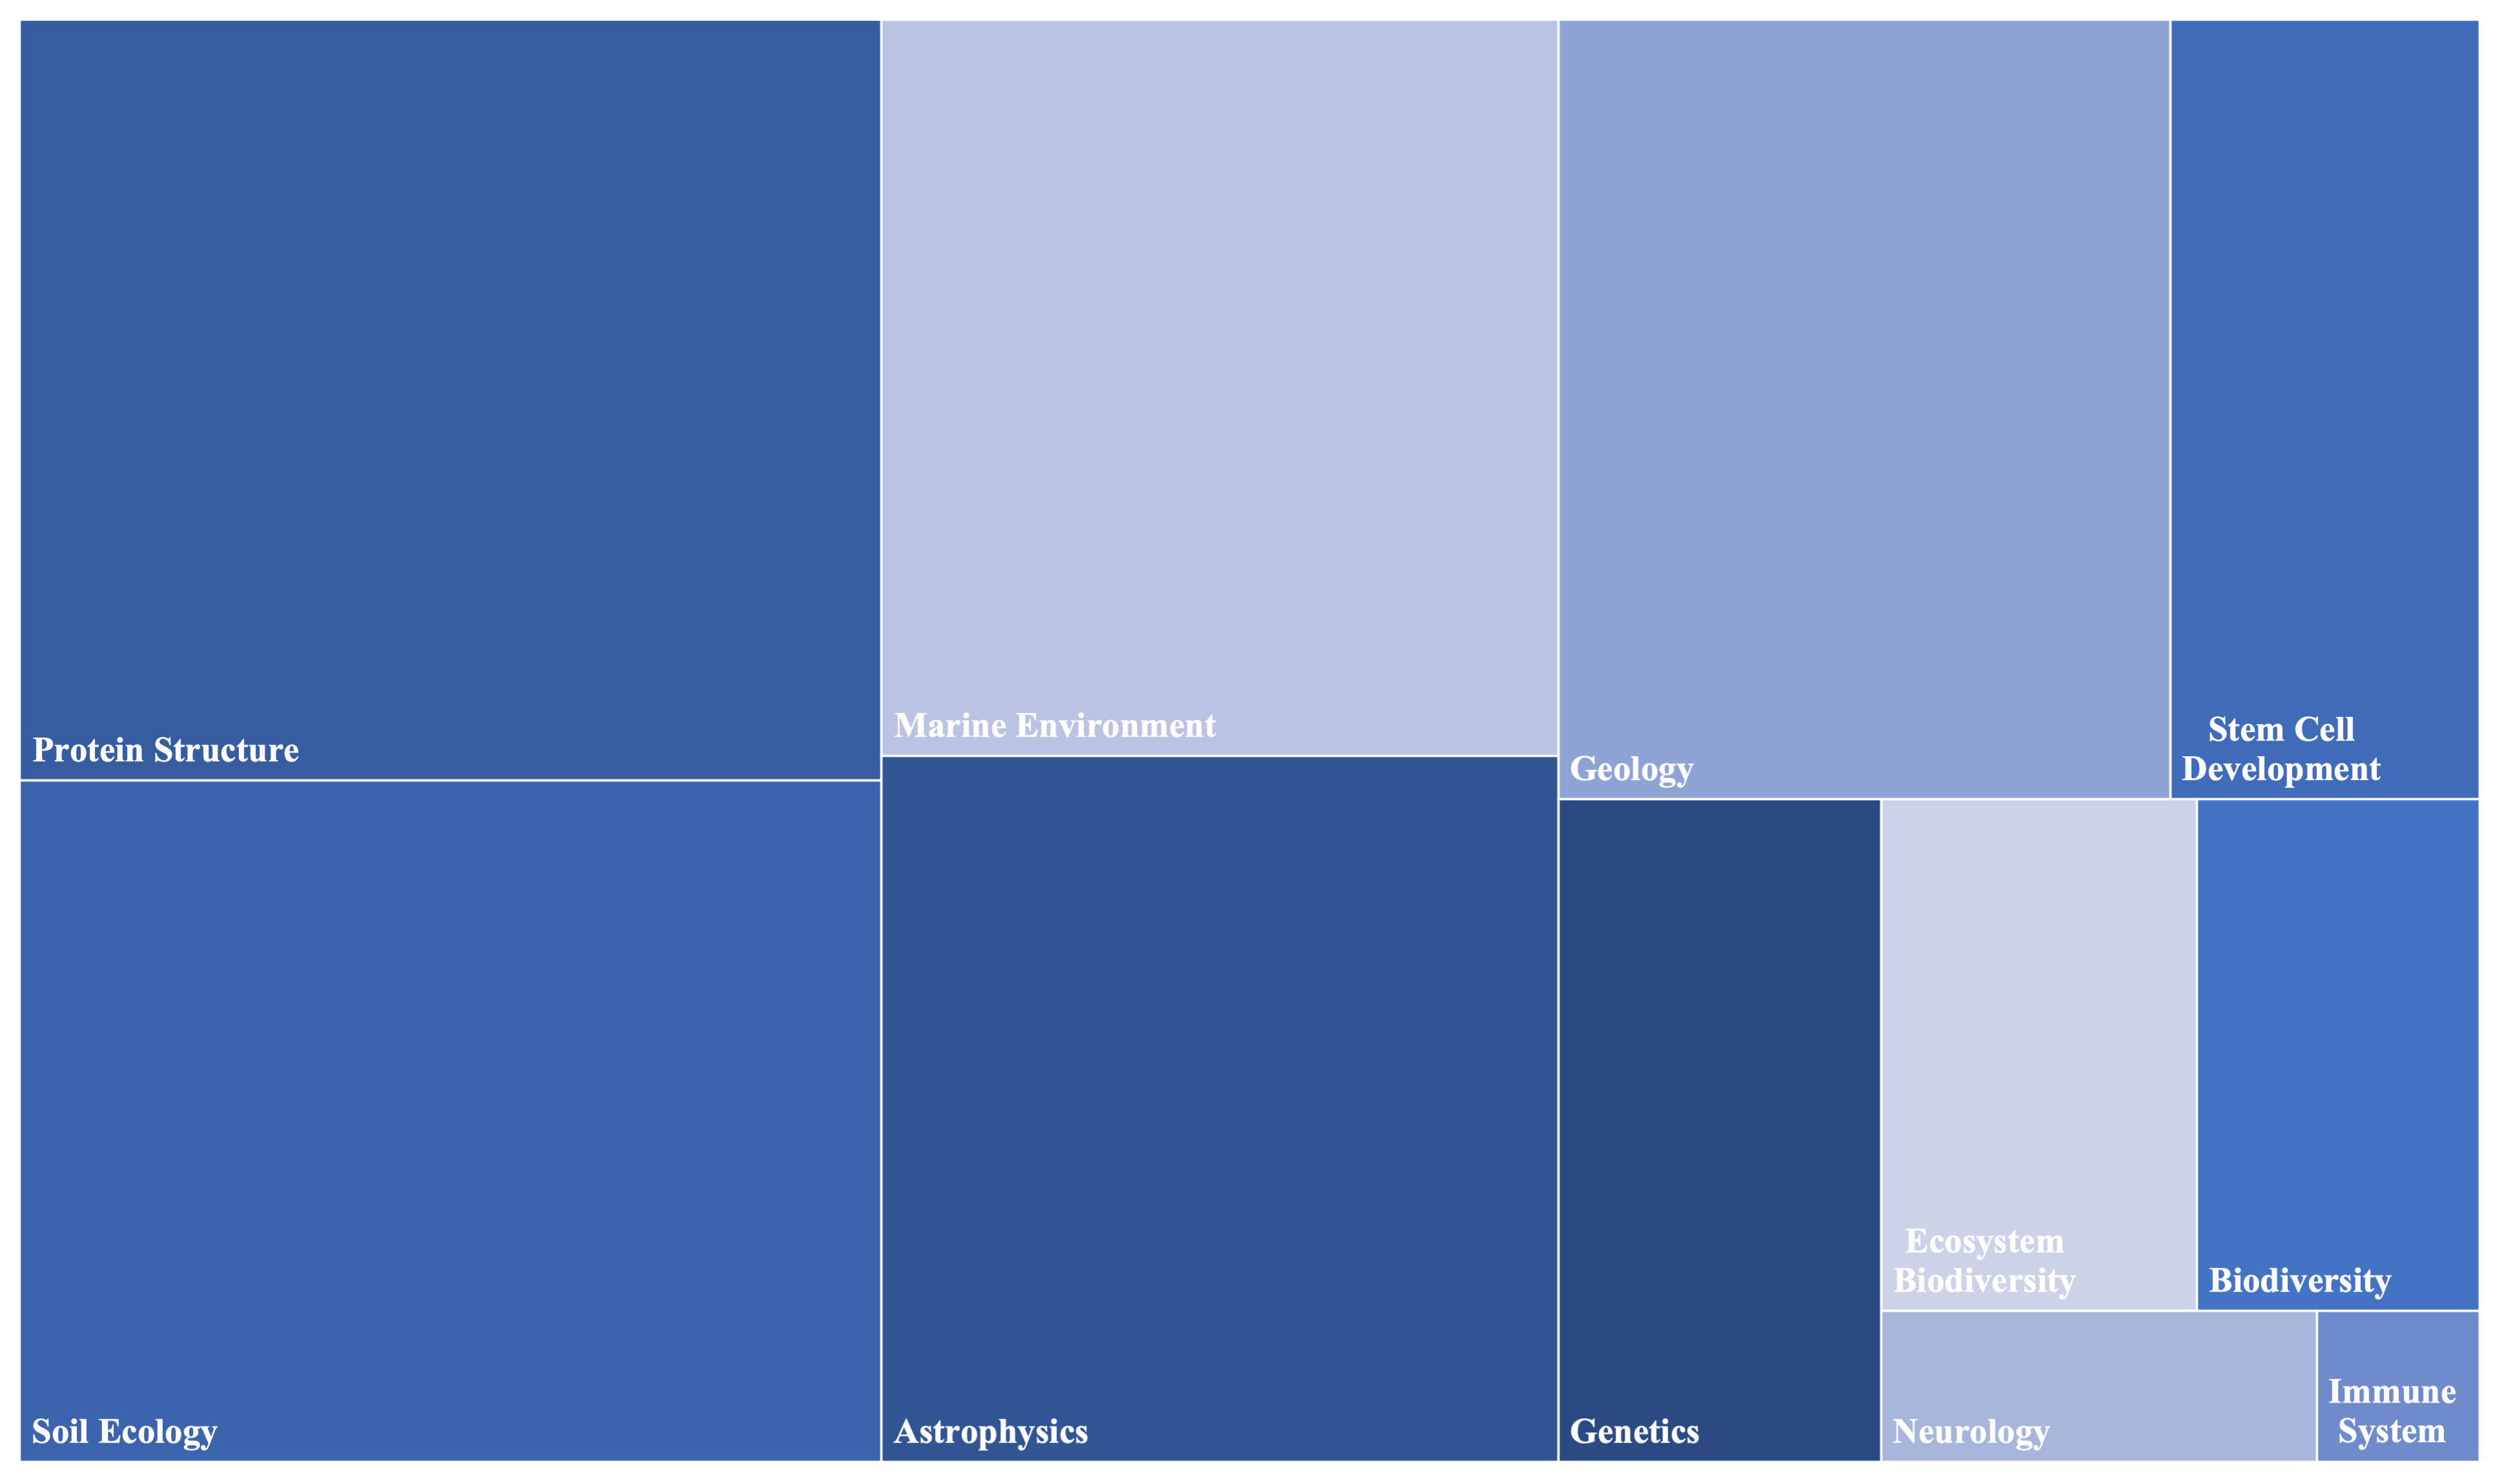
\includegraphics[width=\textwidth]{Figures/Overview of Natural Science Projects Funded in 2019-2021.png}

    \end{subfigure}
    \caption[Investment Directions within Natural Science (2013-2015 and 2016-2018)]{Within the Natural Science category, the field of Life Science consistently received a relatively higher amount of funding compared to Physical Science.}
    \label{fig3.6}
\end{figure}
%TC:endignore
Natural science can be further categorized into two main divisions: life science and physical science. Life science refers to disciplines like biology or human anatomy, essentially encompassing the scientific study of all living organisms on Earth. On the other hand, physical science encompasses the remaining natural sciences, including fields like chemistry and physics, as well as areas unrelated to life \citep{ledoux2002defining}.\\

%TC:ignore
\begin{figure}[H]
\centering
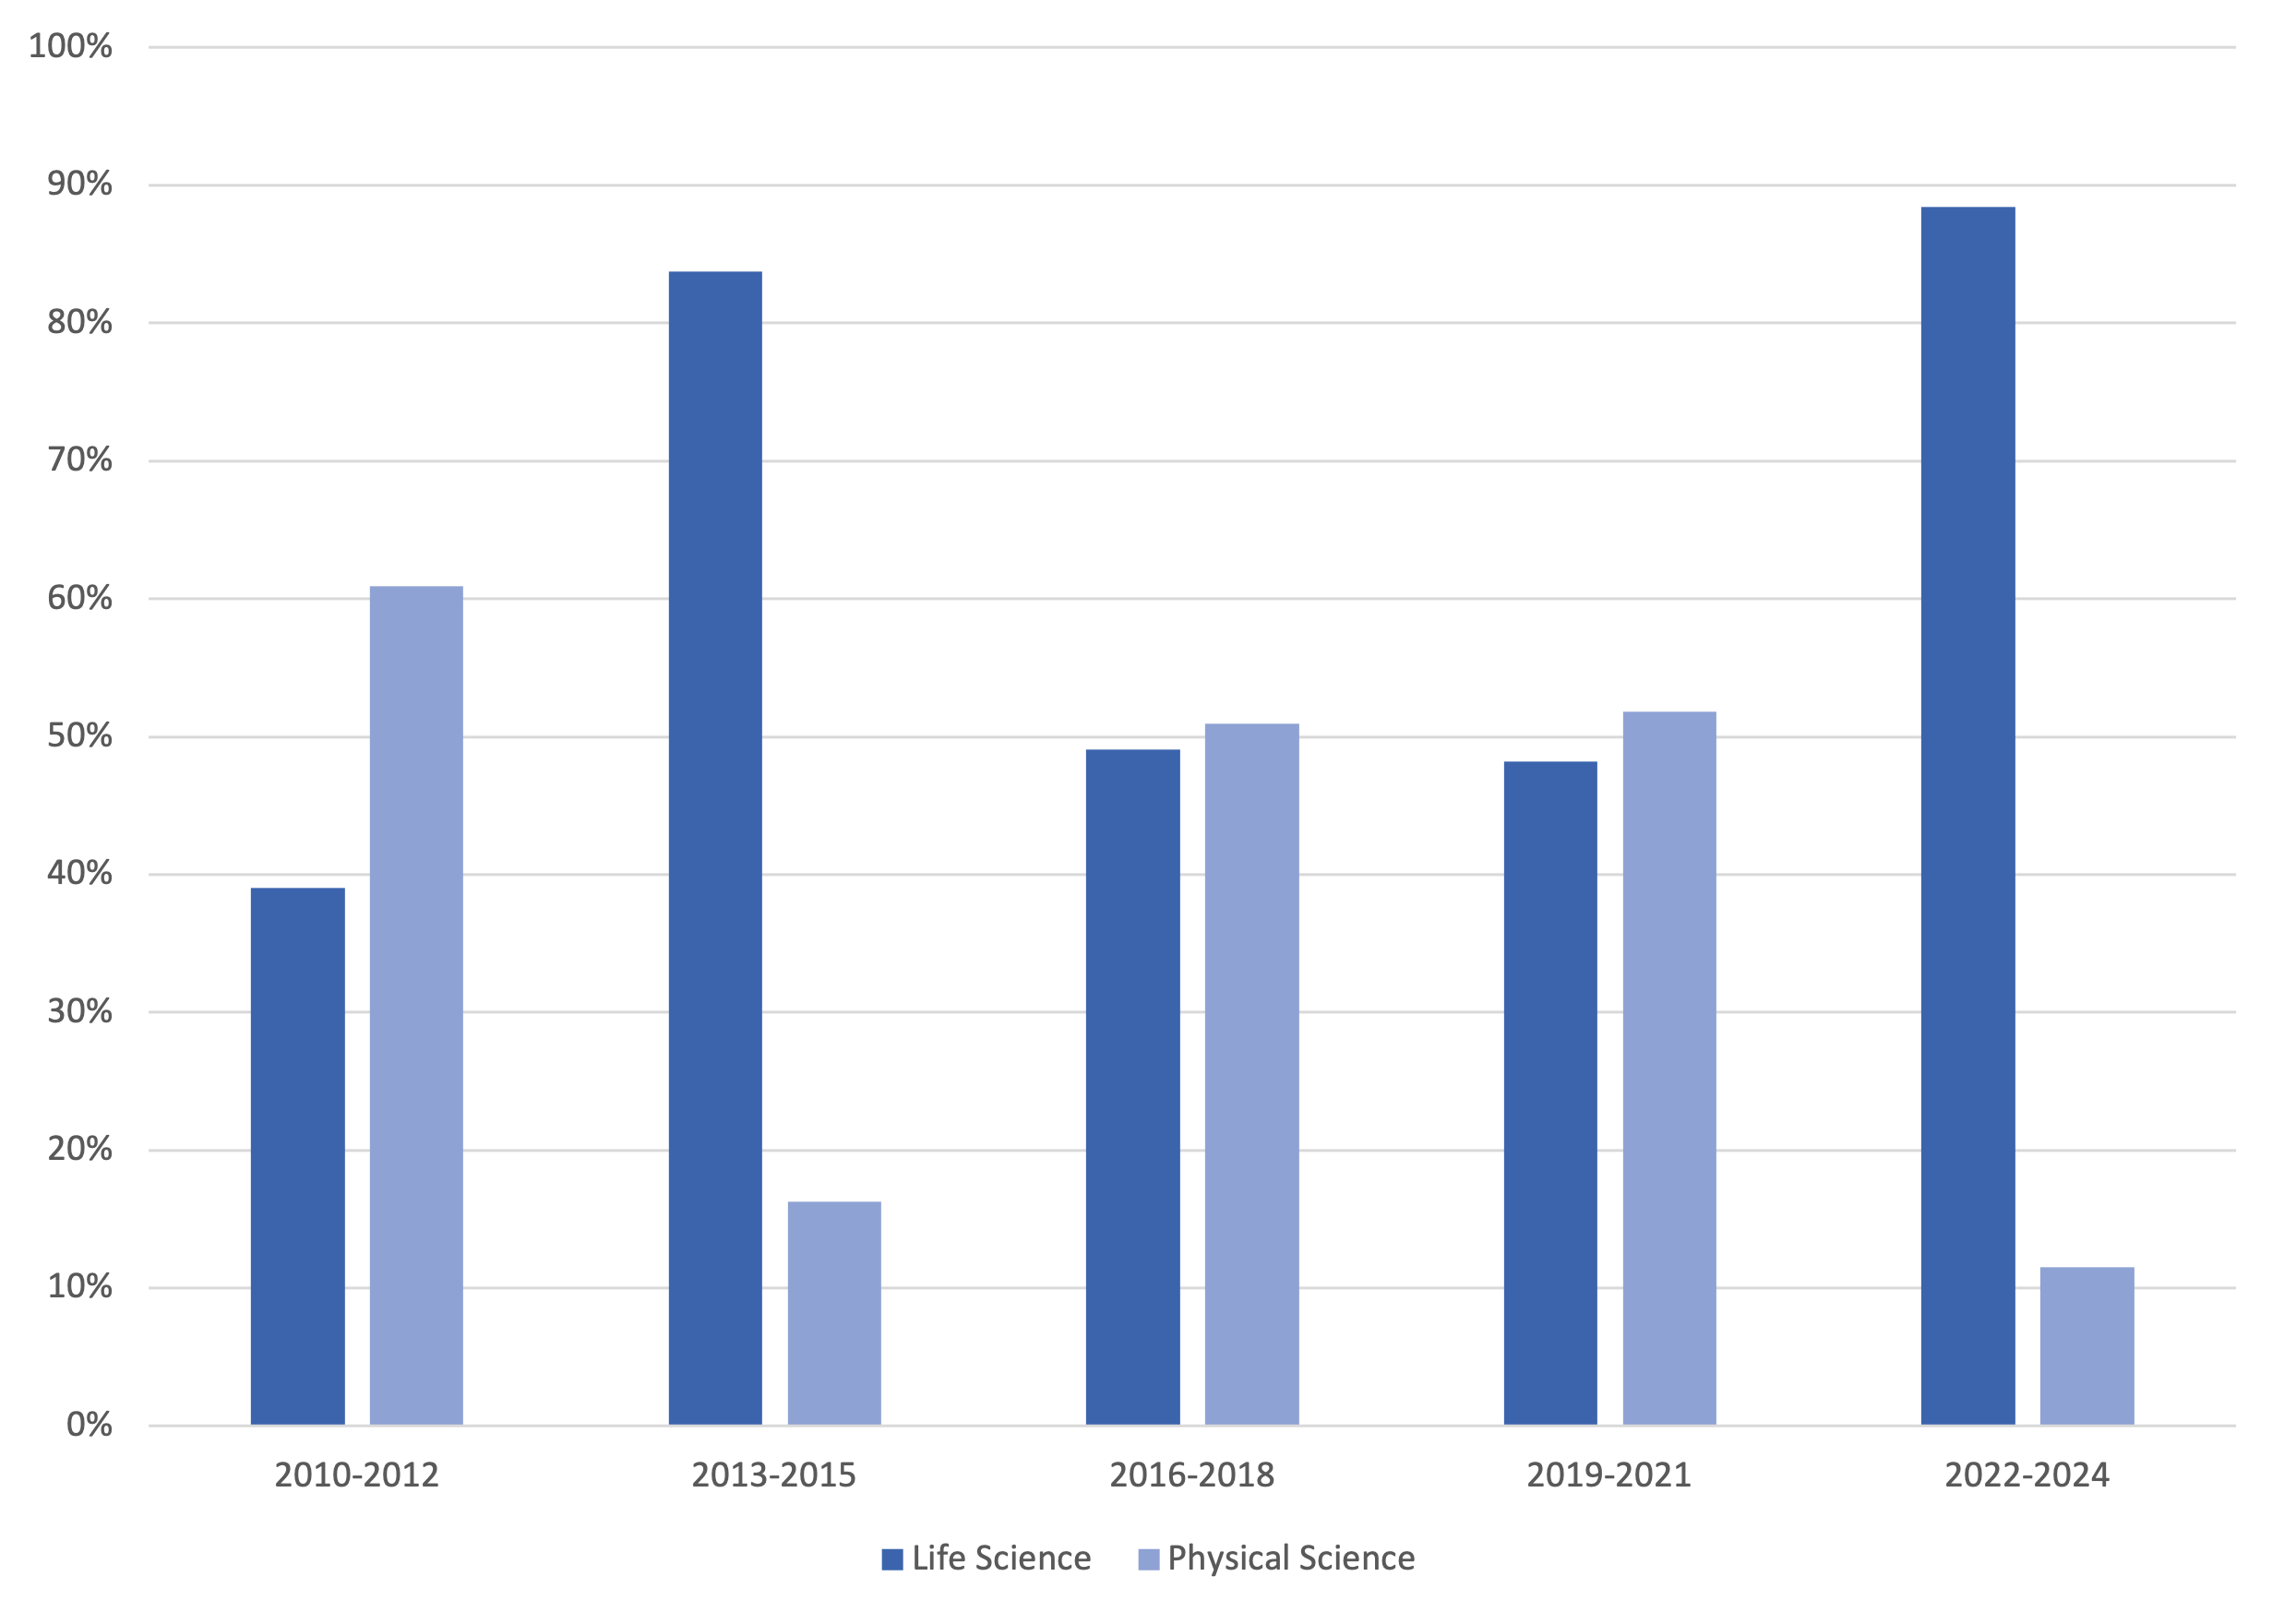
\includegraphics[scale=0.8]{ProjectReportTemplate/Figures/natural_science_prop.png}
\caption[Allocation of Funding in Natural Science]{UKRI does not show a clear preference for either life science or physical science within the category of natural science.}
\label{figure} 
\end{figure}
%TC:endignore

The data for the years 2022-2024 has provided further intriguing insights. UKRI's investment strategy during this period continues to favor natural science and applied science, reflecting a continued emphasis on these domains. Funding for specific sub-disciplines such as Public Health, Computer Science, Fluid Dynamics, and Ecology has also been sustained. However, due to the incompleteness of data for 2023 and 2024, with several projects still in the application phase, a comprehensive analysis of the funding trends for this period has not been conducted. This highlights the dynamic nature of research funding and the ongoing evolution of priorities within the funding landscape. Further investigation into these recent trends may unveil new dimensions of research support and shed light on emerging directions.\\


\section*{Evolution of Funding Amounts in Specific Disciplines}

Continuing our investigation, I delve into the intriguing landscape of disciplines that have consistently secured funding over time. While these disciplines have remained on the funding roster, the allocated amounts have fluctuated, possibly influenced by the specific financial requirements of projects during each period. By delving into these nuances, we aim to discern the intricate patterns underlying funding variations and shed light on the evolving priorities within various domains.\\

%TC:ignore
\begin{table}[H]

    \caption{Consistently Funded Research Topics Across Five Phases (2010-2024)}
    \label{tab: Topic List1}


        \begin{tabular}{ *{4}{c} } 

            \midrule
           Imaging &Genetics &Computer Science&Environmental Science \\
           Pharmaceutical Science&Particle Physics&
           Fluid Dynamics&Education\\
           Geology&Ecology&Public Health &Materials Science\\

            \bottomrule
        \end{tabular}

\end{table}
%TC:endignore

Compared to the Natural Science and Applied Science categories, which have prominently led in the number of funded projects and the allocated amounts, the domains of Social Science and Formal Science exhibit a more stable array of funded research directions. Within Formal Science, fields such as Theoretical Physics and Computer Science have consistently secured funding, reflecting their enduring significance.\\

On the other hand, Natural Science and Applied Science have encompassed a diverse spectrum of funded research domains. Notably, this diversity includes areas like Environmental Science, Ecology, Pharmaceutical Science, and various branches of Biology. Biology has emerged as a dynamic focal point, manifesting a rich tapestry of funded sub-disciplines over the past two decades. These encompass a myriad of specializations, such as Cell Biology, Molecular Biology, Microbiology, and more.\\

Furthermore, "Public Policy" stands as a distinctive current within the realm of Social Science, representing a significant recipient of funding. Notably, within the broader landscape of Social Science, "Public Policy" consistently demonstrates a relatively higher probability of securing funding. This prominence underscores this field's vital role in shaping and informing societal decisions, governance, and strategies.\\

Indeed, the disparity in funding amounts across various domains does not inherently reflect the differing levels of emphasis by UKRI. The allocation of funds is largely influenced by the financial requirements of individual projects. Certain research fields necessitate substantial financial investments due to the costs associated with experimental equipment, while other domains, such as purely theoretical research, might have relatively lower demands for resources.\\


%TC:ignore
\begin{figure}[H]
    \centering
    \begin{subfigure}{\textwidth}
        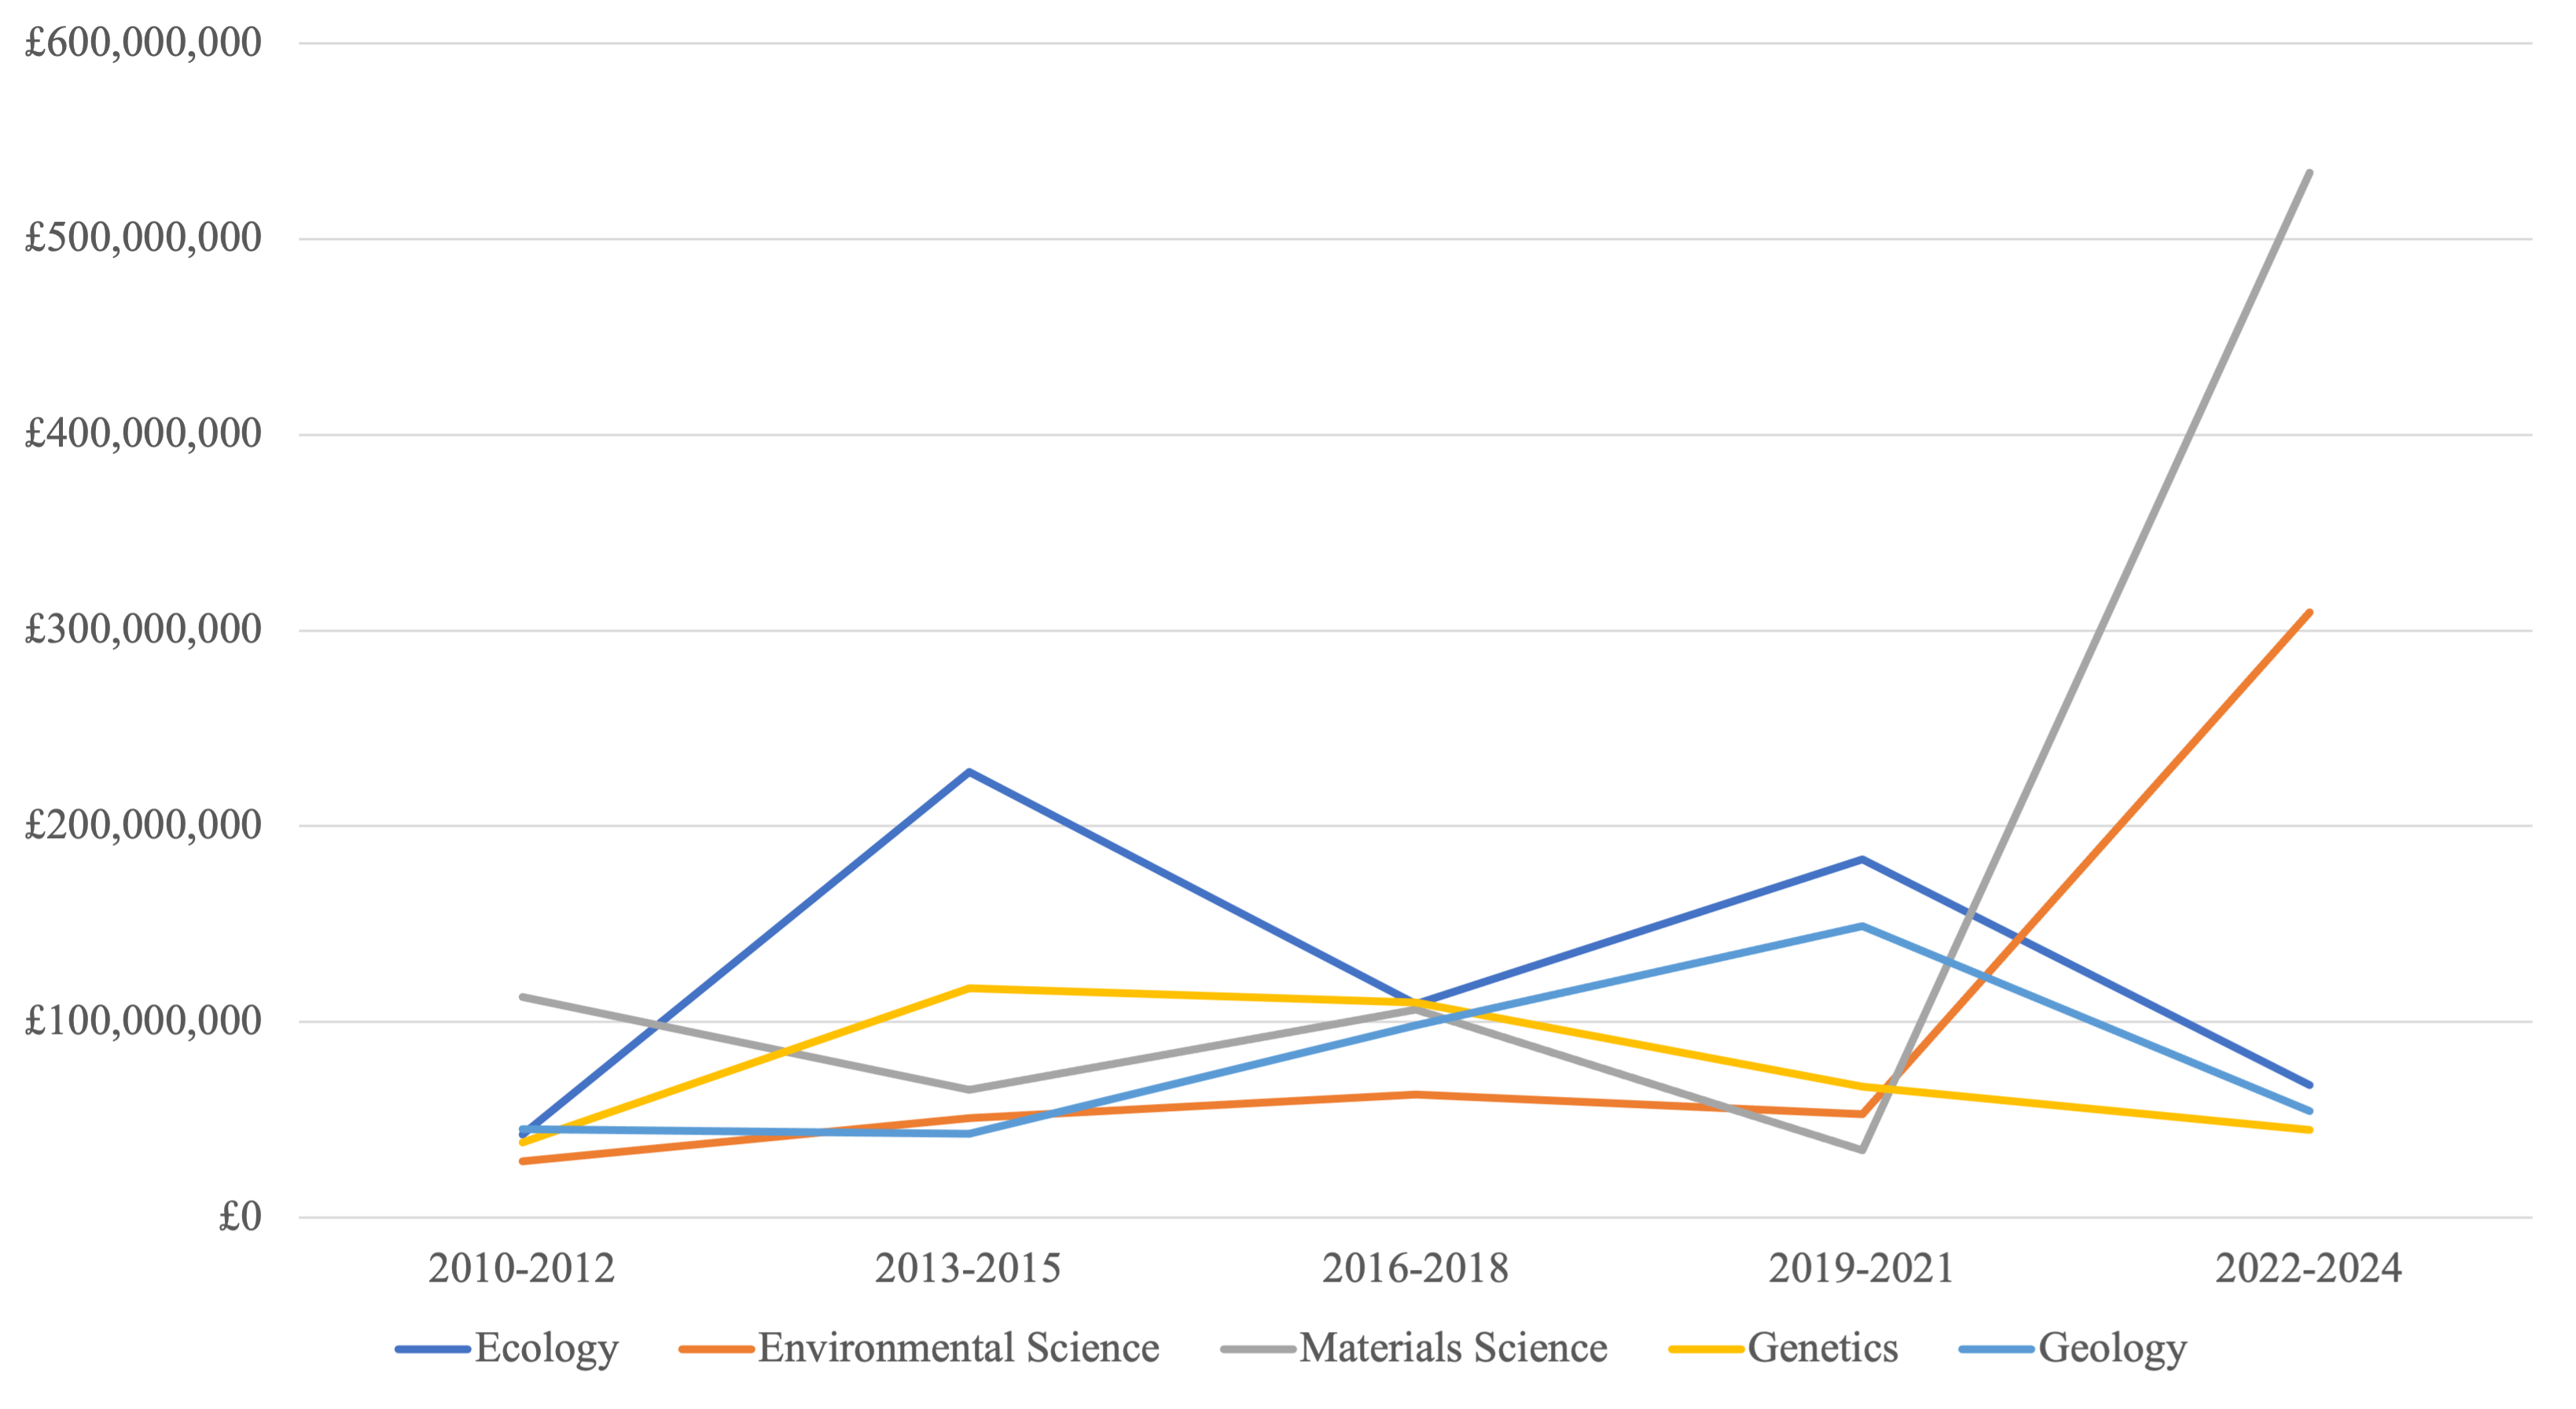
\includegraphics[width=0.8\textwidth]{Figures/Natural Science Funding Trends.png}
       
        \label{fig:2016-2018}
    \end{subfigure}

    \begin{subfigure}{\textwidth}
        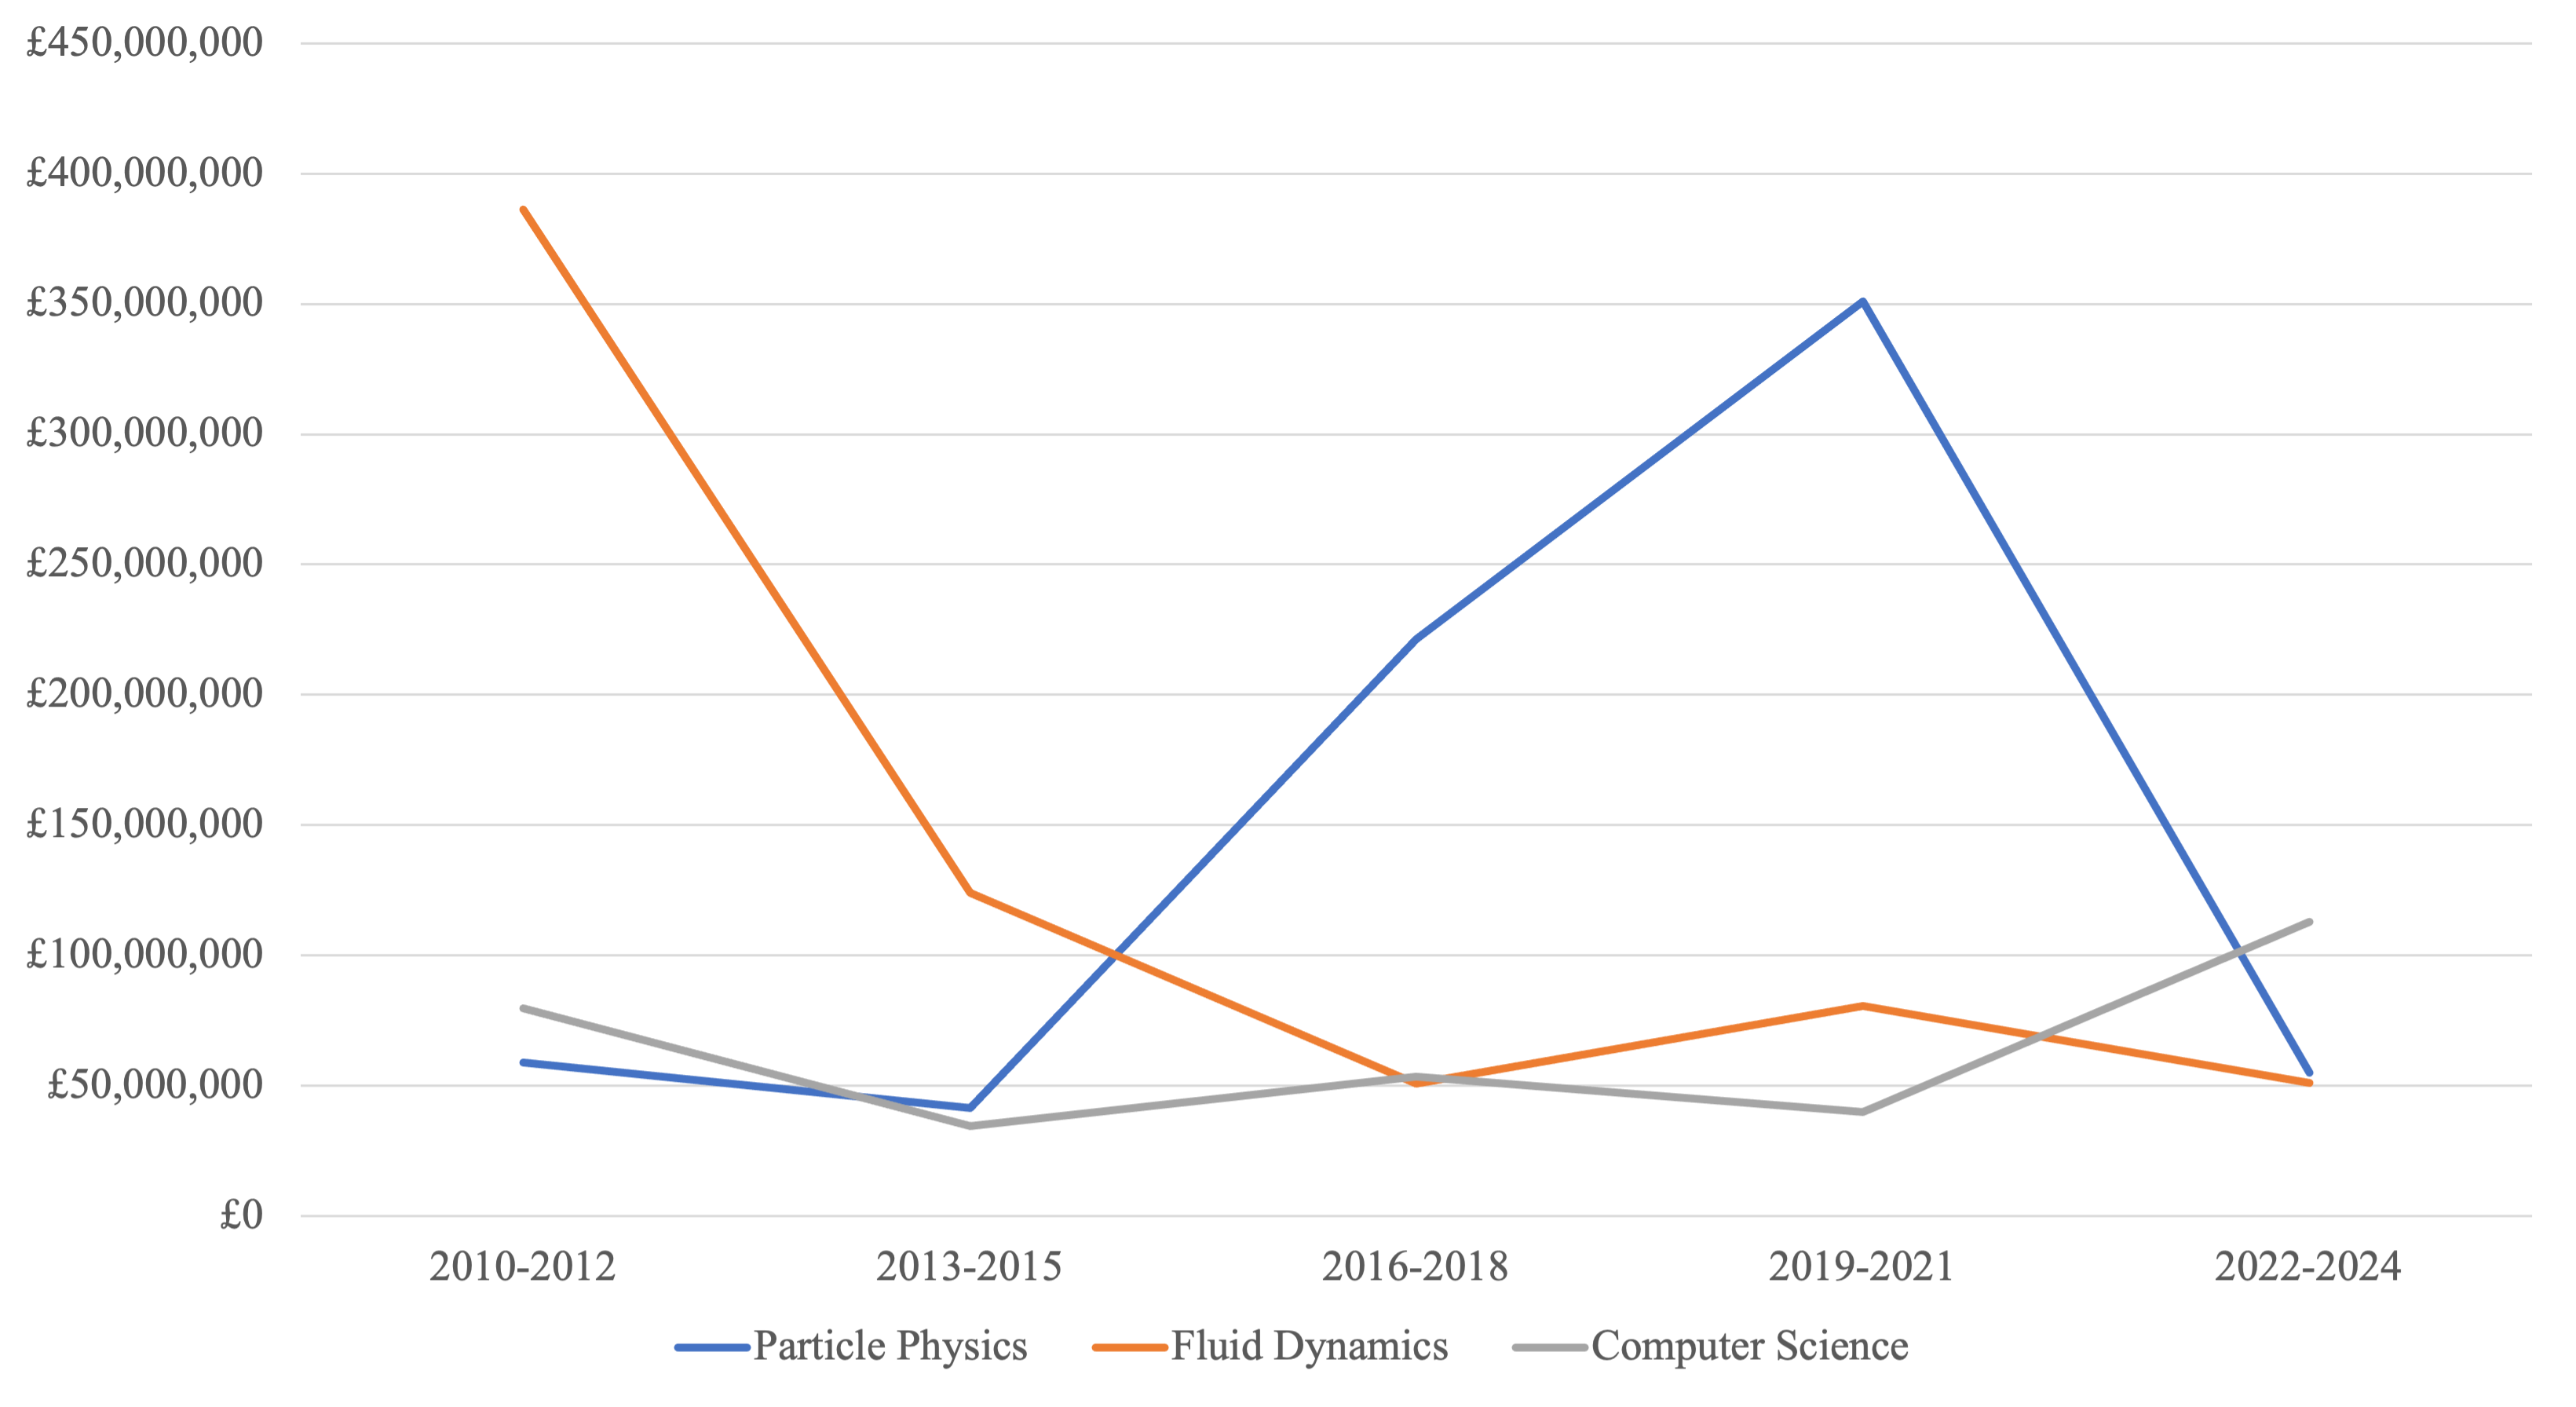
\includegraphics[width=0.8\textwidth]{Figures/Formal Science Funding Trends.png}
       
        \label{fig:2019-2021}
    \end{subfigure}
    \caption[While these directions have received consistent financial support, none of them exhibit a clear growth trend.]{Changing Fortunes in Science Funding}
    \label{fig3.8}
\end{figure}
%TC:endignore

Despite continuous funding support from UKRI over 21 years, there is no discernible consistent pattern in funding amounts for these research directions. Each direction has experienced significant fluctuations in funding levels. Notably, most projects within natural science have consistently received funding around or below 200,000,000. This suggests that while natural science projects contribute to the overall funding pool, the allocation per individual direction remains relatively modest. Within this context, it is worth highlighting that ecology has consistently outperformed other directions in terms of funding amounts, indicating promising prospects for the field.\\


\chapter{Discussion}
\lettrine[lines=1]{V}{arious}
factors guide the decisions different countries make regarding science funding allocation. The anticipated outcomes of this project's research are evident in many cases. Many disciplines within the natural and applied sciences rely heavily on funding, with substantial investments required for experimental materials and equipment. Moreover, the results generated within these two domains are more readily applicable, yielding greater economic advantages.\\

In contrast, formal sciences and many social science disciplines lean towards advancing our fundamental understanding of nature rather than providing information directly applicable in practical contexts \citep{shaw2022revisiting}. This propensity often results in fewer institutions funding research due to limited immediate tangible benefits. Apart from economic considerations, funding decisions are increasingly subject to external pressures. The demand for societal relevance may influence expert panel perceptions of research quality. Some researchers even express concerns that institutional assessments such as the "Research Excellence Framework" in the UK could adopt criteria that ultimately become ineffective substitutes for gauging research quality \citep{meirmans2019science}.\\

In this context, fields such as public health, computer science, ecology, fluid dynamics, biology, and pharmaceutical science have emerged as popular and well-funded domains, and the factors driving this sustained support are multifaceted. Firstly, in the post-pandemic era, the prominence of public health, pharmaceutical science, and biology can be attributed to their widespread societal demand and profound impact. Particularly, research in public health encompasses human well-being and disease prevention, directly influencing overall societal health and quality of life. Simultaneously, against the backdrop of escalating environmental pollution and climate change concerns, research in environmental science, ecology, materials science, and sustainable energy holds crucial significance for environmental preservation and ecological equilibrium. Additionally, computer science plays a pivotal role in digitization, exerting substantial influence on technological innovation, information technology, and data analytics.\\

Moreover, the research and applications within these fields directly address numerous real-world challenges. Especially in the current era of advanced artificial intelligence, computer science is a foundational discipline underpinning the profound development of emerging fields. As a fundamental scientific field, the continuous funding support for fluid dynamics further underscores the UK's commitment to international competitiveness and influence.\\

In addition, the research has also yielded some unforeseen outcomes. For instance, the substantial investments made by UKRI in the environmental and renewable energy sectors during 2016-2018, as well as the stark contrast between the increasing number of projects receiving investments in the applied science domain and the diminishing investments in certain specific subfields. The heightened focus on environmental concerns during this period could be attributed to the historical milestones of 2016, marked by record-breaking global temperatures, diminished polar ice, rising sea levels, and escalating ocean heat content. The persistence of extreme weather events and climatic conditions into 2017 drew global attention, potentially influencing UKRI's decision-making processes.\\

Furthermore, the aggregated nature of investments in the applied science domain might reflect UKRI's inclination towards channels that have been previously funded. Continuous investments in domains such as Medical Technology, Agricultural Science, and Immunology may signify positive developments in these fields, suggesting ongoing advancements or the likelihood of breakthrough progress in the near future.\\


Furthermore, with the rapid development of artificial intelligence and platforms like ChatGPT in recent years, the pervasive impact of AI across diverse sectors of the internet has garnered widespread attention. The dynamic evolution of AI technologies and modeling techniques is noteworthy. It is reasonable to anticipate a potential increase in funding or the number of projects in AI, modeling, and related fields.\\


\section*{Limitation}
Certainly, given the incompleteness of data for the years 2022-2024, it is essential to acknowledge that the current analysis comes with limitations and potential biases stemming from pending projects still in the application phase. However, from my perspective, the emphasis on addressing environmental pollution and promoting public health has been consistently evident. As a result, fields related to environmental concerns and various branches of biology remain focal points for funding allocation.\\

\section*{Conclusions}
In the intricate landscape of science funding allocation, the decisions made by different countries are guided by a complex interplay of factors. This study unveiled various trends and considerations that shape funding distribution across different scientific domains. Notably, funding allocation is multifaceted, influenced by societal demands, economic advantages, and research relevance. While applied and natural sciences often garner substantial funding due to their practical applications and economic benefits, formal sciences and certain social science disciplines focus on advancing fundamental understanding rather than immediate practicality.

Public health, computer science, ecology, fluid dynamics, and pharmaceutical science have emerged as well-funded and impactful domains. The pandemic has underscored the importance of public health and pharmaceutical research, while environmental concerns and technological advancements have driven investments in ecology, sustainable energy, and computer science.


In conclusion, science funding allocation is a dynamic process influenced by many factors. The trends identified in this study reflect a balance between societal needs, economic considerations, and research objectives. With its ever-changing challenges and opportunities, the evolving scientific landscape will continue to shape funding priorities and drive innovation in the years to come.


\section*{Data and Code Availability}
The original dataset for this project can be obtained from https://www.dropbox.com/scl/fo/x85cc5gxk8uxu5x1c5lpz/h?rlkey=5ryaw51zilehxhisyah7prt4u&dl=0. The corresponding source code is available at https://github.com/hyjiang0120/MappingFunding.

\nolinenumbers

% Add other chapters if and when need be.

\newpage
\nocite{*}
\renewcommand{\bibname}{References}
\phantomsection
\addcontentsline{toc}{chapter}{References}
\bibliography{Content/citation}

\end{document}